\documentclass[11pt]{scrartcl}
\usepackage[sexy]{evan}
\usepackage{graphicx}

 %Sets
\newcommand{\N}{\mathbb{N}}
\newcommand{\Z}{\mathbb{Z}}
\newcommand{\F}{\mathbb{F}}
\newcommand{\Q}{\mathbb{Q}}
\newcommand{\R}{\mathbb{R}}
\newcommand{\C}{\mathbb C}
\newcommand{\T}{\mathbb T}
\newcommand{\SRS}{\mathscr {S}}

\let \phi \varphi
\let \hat \widehat

\newcommand{\<}{\langle}
\renewcommand{\>}{\rangle}

%From Topology
\newcommand{\cT}{\mathcal{T}}
\newcommand{\cB}{\mathcal{B}}
\newcommand{\cC}{\mathcal{C}}
\newcommand{\cH}{\mathcal{H}}


\usepackage{answers}
\Newassociation{hint}{hintitem}{all-hints}
\renewcommand{\solutionextension}{out}
\renewenvironment{hintitem}[1]{\item[\bfseries #1.]}{}
\declaretheorem[style=thmbluebox,name={Theorem}]{thm}

\begin{document}
\title{Math 258}
\author{Vishal Raman}
\thispagestyle{empty}
$ $
\vfill
\begin{center}

\centerline{\huge \textbf{Math 258 Lecture Notes, Fall 2020}}
\centerline{\Large \textbf{Harmonic Analysis} } 
\centerline{Professor: Michael Christ}
\centerline{Vishal Raman}
\end{center}
\vfill
$ $
\newpage
\thispagestyle{empty}
\tableofcontents
\newpage
%\maketitle
\section{August 27th, 2020}
\subsection{Introduction}
We begin by considering the problem of conduction of heat in a circle.  We use the map $x \mapsto e^{ix}, x \in [0, 2\pi)$.  Where $u$ is the temperature, $t$ is the time, we believed that $u_t = \gamma u_{xx}$, where subscripts denote partial derivatives.  We also have an initial condition, $f(x) = u(x, 0)$.

There are some simple solutions $e^{inx}e^{-\gamma n^2t}|_{t=0} = e^{inx}$.  The product of solutions, the sum of solutions, and scalar multiple of solutions are all solutions, so he wrote the solution as $$f(x) = \sum_{n = -\infty}^{\infty} a_n e^{inx}, u(x, t) = \sum_{n} a_n e^{-\gamma n^2t}e^{inx}.$$

\subsection{Fourier Analysis}
We take a circle $\{z \in \C : |z = 1|\}$, which can also be thought of as $\R/(2\pi\Z)$, with the map $x \mapsto e^{ix}$. 
 Suppose we have $G$ a finite abelian group, and $\hat{G} = \{\text{hom }\phi:G \rightarrow \R/\Z \}$, the dual group.  $\hat{G}$ is also a group, formally known as the set of characters.

\begin{example} If we take $G = \Z_N = \Z/N\Z$, with the map $x \mapsto e^{2\pi i xn/N}$, for $n \in Z_n$.

 Similarly, taking $G \cong Z_{N_1} \times \Z_{N_2} \times \dots$, we take $x \mapsto \prod e^{2\pi i xn/N_i}$.
\end{example}

Take $e_\xi(x) = e^{2\pi i \xi(x)}$, where $\xi: G \mapsto \R/\Z$.  Working in $L^2(G)$, we note the following:

\begin{fact} If $\xi \ne \varphi$, then $\left<e_\xi, e_\varphi \right> = 0$.
\end{fact}
\begin{proof}
$$\sum_{x \in G} \xi(x) \overline{\varphi(x)} = \sum_{u} \xi(u+y)\overline{\varphi(u+y)} - \left (\sum_u \xi(u)\overline{\varphi(u)}\right ) \xi(y) \overline{\varphi(u)}.$$
Hence, either $\left < \xi, \phi\right > = 0$ or $\xi(y)\overline{\phi}(y) = 1$ for all $y \in G$, which implies $\xi = \phi$.
\end{proof}
If follows that $\{e_f : f \in \hat{G}\}$ is an orthonormal set in $L^2(G)$ Then, the dimension is $|\hat{G}| = |G| = \dim(L^2(G))$.  Hence, the set forms an orthonormal basis for $L^2(G)$.

Then, for all $f \in L^2(G)$,  we have $$\|f\|_{L^2(G)}^2 = \sum_{\phi \in \hat{G}} |\left <f, e_\xi\right >|^2,$$
$$f = \sum_{e_{\xi} \in \hat{G}} \left <f , e_{\xi}\right >e_\phi.$$

\subsection{On Tori of Arbitrary Dimension}
We define $\T = \R/2\pi\Z$, from $[0, 2\pi]$.  We then work on $\T^d$, $d \ge 1$.  

For $f \in L^2(\T^d)$, we define $$\hat{f}(n) = (2\pi)^{-d}\int f(x)e^{-inx}dx.$$

We have an inner product $\left <f, g\right > = \int_{\T^d} f(x) \overline{g(x)}d\mu(x)$ defined over a Lebesgue measure or Euclidean measure on $\T^d$. 

\begin{thm}[Parseval's Theorem] For all $f \in L^2(\Pi^d)$,
$$\|f\|_{L^2}^2 = (2 \pi)^d \sum_{n \in \Z^d}|\hat{f}(n)|^2,$$
and we have 
$$f = \sum_{n \in \Z^d} \hat{f}(n)e^{inx},$$ in the sense that 
$$\|f - \sum_{n \in \Z^d} \hat{f}(n)e^{inx}\|_L^2 \rightarrow 0.$$ 
\end{thm}
Note: you can usually figure out the constant with the simplest example, $f = 1$.  
\begin{proof}
Take $\T^d, e_n(x) = e^{in\cdot x}$.  The $\{(2\pi)^{-d/2}e^n:n \in \Z^d\}$ is orthonormal(left as an exercise).  Then, for all $f$, $\sum_{n} \left <f, (2\pi)^{-d/2} e_n\right > \le \|f\|_{L^2}^2$, with equality if the set is a basis(Bessel's inequality).  

It suffices to show that $\text{span}\{e_n\}$ is dense in $L^2$.  Take $P = \text{span}\{e_n\}$, and note that $P$ is an algebra of continuous functions on $\Pi^d$,  closed under conjugation, contains $1$, and separates points.  Hence, the Stone-Weierstrass theorem implies that $P$ is dense in $C^o(\Pi^d)$ with respect to $\|\cdot\|_{C^o}$.  Then $C^o \subset L^2$ is dense(general theory about Compact Hausdorff spaces, Radon Measures).  

The statement $\|f - \sum_{n \in \Z^d} \hat{f}(n)e^{inx}\|_L^2 \rightarrow 0$ follows from the general theory of orthonormal systems.
\end{proof}

\subsection{Euclidean Spaces}
We work in $\R^d, (d \ge 1)$.  Take $\xi \in R^d$, and $x \mapsto x\xi \in \R$ is a homomorphism from $\R^d \rightarrow \R$, but if we take $x \mapsto e^{ix\xi}$, we have a homomorphism from $\R^d\mapsto \Gamma$.  We try to define the following:
$$\hat{f}(\xi) = \int_{\R^d} f(x)e^{-ix\xi}dx = \left <f, e_{\xi}\right >_{L^2(\R^d),}$$
where $e_{xi}(x) = e^{ix\xi}$.

Some problems:
\begin{enumerate}
\item $e_\xi \not \in L^2(\R^d)$
\item $f(x)e^{-ix\xi}$ need not be in $L^1$ if $f \in L^2$.
\end{enumerate}
We fix this by imposing extra conditions.
\begin{definition} For $f \in L^1(\R^d)$, we define
$$\hat{f}(\xi) = \int_{\R^d} f(x)e^{-ix\xi}dx.$$
\end{definition} 

Note that $f \in L^1$ implies that $\hat{f}$ is bounded, continuous.  We see this as follows:
$\hat{f}(\xi + u) - \hat{f}(\xi) = \int f(x)e^{-ix\xi}(e^{-ixu}-1)dx$.  If we let $u \rightarrow 0$, the right goes to $0$ pointwise, and $(2|f|) \in L^1$ dominates the integral, it goes to $0$.  
\begin{proposition}If $f \in L^1 \cap L^2(\R^d)$, $\hat{f}\in L^2(\R^d)$, 
$$\|\hat{f}\|_{L^2}^2 = (2\pi)^d \|f\|_{L^2}^2.$$
\end{proposition}

\begin{thm}[Plancherel's Theorem] $\pi: L^1\cap L^2 \rightarrow L^2$ extends uniquely to $\hat{\pi}: L^2(\R^d) \rightarrow L^2(\R^d)$, linear, bounded, 
$\|\hat{\pi}f\|_{L^2}^2 = (2\pi)^d\|f\|_{L^2}^2$,
and for all $f \in L^2$, we have an inverse Fourier Transform,
$\check{f}(y) = \int f(\xi)e^{iy\xi}d\xi$ for $f \in L^1 \cap L^2$, and $\check{\cdot}$ also extends.  

Finally, $$\|f - (2\pi)^{-d}\int_{|\xi| \le R} \hat{f}(\xi)e^{ix\xi}d\xi\|_{L^2} \rightarrow 0.$$
\end{thm}
Note that $\check{f}(y) = \hat{f}(-y)$.
\begin{proof}
We first prove that $\|f\|_{L^2}^2 = (2\pi)^{-d}\|\hat{f}\|_{L^2}^2$ for all $f \in L^1 \cap L^2$.  We prove this for a dense subspace $\mathscr{P} $ of $L^2$.  We will show later that there exists a subspace $V \subset L^2(\R^d)$ so that $V$ is dense in $L^2$, $V \subset L^1$, $\forall f \in V,$ there exists $C_f < \infty$, so for all $\xi \in \R^d$, $|\hat{f}(\xi)| \le C_f(f(\xi))^{-d}$ and $f$ is continuous with compact support.

We are given $f: \R^d \rightarrow \C$ supported where $|x |\le R = R_f < \infty$.  For large $t \ge 0$, define $f_t(x) = f(tx)$(this shrinks the support of $f$), supported where $|x| \le R/t < \pi$.  We can then think of $f_t: \T^d \rightarrow \C$.  

Now, we calculate
\begin{align*}
\hat{f}_{t}(n) & = (2\pi)^d\int_{\T^d} f_t(x)e^{-inx}dx\\
&= t^{-d}(2\pi)^d \int_{R^d} f(x)e^{-in/ty}dy \\
&= t^{-d} (2\pi)^{-d}\hat{f}(t^{-1}n),
\end{align*}
where the first hat is on $\T^d$ and the second is on $\R^d$, so the Fourier coeficients in the euclidean case are scalar multiples of the Fourier coefficients in the Tori case.  

Thus,
$$\|f_t\|_{L^2(\T^d)}^2 = t^{-d}\|f\|_{L^2(\R^d)}^2 = c_d\sum_{n \in \Z^d}|\hat{f}_t(n)|^2 = c_d't^{-2d}\sum_{n} |\hat{f}(t^{-1}n)|^2$$

Hence,
$$\|f\|_{L^2(\R^d)}^2 = c_d't^{-d}\sum_{n} |\hat{f}(t^{-1}n)|^2.$$

This has a nice tiling Riemann sum interpretation: if we take $\R^d$ and tile it with cubes of sidelength $1/t$ where one corner is at $t^{-1}n$ for $n \in \Z^d$, then
$$\|f\|_{L^2(\R^d)}^2 = c_d' t^{-d}\sum_{n}\left |\hat{f}(t^{-1}n)\right |^2 = \int_{\R^d}|g_t|^2 dx,$$
where $g(x) = \hat{f}(t^{-1}n)$.
 
We claim 
$$\int_{\R^d}|g_t|^2 \rightarrow \int_{\R^d}|\hat{f}|^2,$$
which follows from the dominated convergence theorem:  where we take a sequence over $t$ going to infinity, with dominator $C_f^2(1 + |\xi|)^{-2d}$ in $L^1$ and $|\hat{f}(\xi)| \le C_f^2(1 + |\xi|)^{-2d}$. Furthermore, we have $g_t(\xi) \rightarrow \hat{f}(\xi)$ as $t \rightarrow 0$, and $\hat{f}$ is continuous so $g_t$ is pointwise convergent, and we have
$$|g_t(\xi)| = |\hat{f}(t^{-1}n)| \le C_f(1 + |t^{-1}n|)^{-d} \le C'(1 + |\xi|)^{-d}.$$
\end{proof}
\newpage
\section{September 1st, 2020}
\subsection{Proof of Plancherel's Theorem}
Last time
\begin{itemize}
\item $\R^d$, $$\hat{f}(\xi) = \int_{\R^d} e^{-ix \cdot \xi} f(x)dx.$$
\item $V = (f \in L_1 \cap L_2(\R^d)) : |\hat{f}(\xi)|\left <\xi \right >^d$ is a bounded linear function, $\left< x\right > = (1 + |x|^2)^{1/2} \ge 1, = |x|$ for $x$ large.
\item Claim: $V$ is dense in $L^2(\R^d)$.  Then $\|\hat{f}\|_{L^2} = (2\pi)^{d/2}\|f\|_{L^2}$ for all $f \in V$ so there exists a unique bounded linear operator $\mathscr{F}$ on $L^2(\R^d)$, where $\mathscr{F}$ takes a function to it's fourier transform.
\item We discussed some properties of $\mathscr{F}$.
\begin{itemize}
\item $\|\mathscr{F}f\|_2 = (2\pi)^{d/2} \|f\|_2$
\item $\mathscr{F}$ is onto.
\item For all $f \in L^2$, $$\left\|f - (2\pi )^{-d} \int_{|\xi| \le R}e^{ix \cdot \xi}\mathscr{F}(f)(\xi) d\xi \right \|_{L^2}\rightarrow 0,$$
in the limit where $R \rightarrow \infty$.
\end{itemize}
\end{itemize}
First note that $\mathscr{F}$ has closed range(this was an exercise).  It suffices to show: If $g \in L^2, g \perp \mathscr{F}(f) $ for all $f \in V$, then $g = 0$.
\begin{proof} First, note that 
$$0 = \left <g, \mathscr{F}(f)\right >= \left <\mathscr{F}^*(g),f\right >,$$ 
and for all $g \in V$, $$\mathscr{F}^*g(x) = \int g(\xi)e^{ix \cdot \xi}d\xi$$
Therefore, $\mathscr{F}^*(g)(x) = (\mathscr{F}g)(-x)$ for all $g \in V$, which is dense in $L^2$.  Hence, $\mathscr{F}g = 0$, and the Fourier transform preserves norms, so $g = 0$.
\end{proof}
We also claimed the following:
Let $f \in L^2$:
$$\|f(x) - (2\pi)^{-d}\int_{|\xi| \le R} (\mathscr{F}f)(\xi)e^{ix\cdot \xi}d\xi\|_2^2 \rightarrow 0.$$
\begin{proof}
Let $g_r = (2\pi)^{-d}\int_{|\xi| \le R} (\mathscr{F}f)(\xi)e^{ix\cdot \xi}d\xi$.We have to show $\langle f, g_r \rangle \rightarrow \|f\|_2^2$.  Then
$$\|f - g_r\|_2^2 = \|f\|_2^2 + \|g_r\|_2^2 - 2 \text{Re}\langle f, g_r \rangle \rightarrow \|f\|_2^2 + \|f\|_2^2 - 2 \|f\|_2^2.$$
\begin{align*}
\left <f, g_R\right > &= (2\pi)^{-d} \int f(x) \overline{\int_{|\xi| \le R} (\mathscr{F}f)(\xi)e^{ix \cdot \xi}d\xi} dx\\
&= (2\pi)^{-d} \int_{|\xi| \le R} \left (\int f(x)e^{-ix \cdot \xi} dx\right ) \overline{(\mathscr{F}f)(\xi) d\xi}\\
&= (2\pi)^{-d} \int_{|\xi| \le R} |\mathscr{F}f(\xi)|^2 d\xi \rightarrow (2\pi)^{-d} \|\mathscr{F}f\|_2^2 = \|f\|_2^2.
\end{align*}
However, it's not clear that we can use Fubini's theorem.  We would need $f \in L^1 \cap L^2$.  But this is not an issue as $L^1 \cap L^2 \subset L^2$ is dense, so if we let $\epsilon > 0, f = G+h, \|h\|_2 \le \epsilon$ and $G \in L^1 \cap L^2$.  Showing the convergence from here is an exercise.
\end{proof}
We still need $V = (f \in L^1 \cap L^2 : \left <\xi\right>^d (\hat{f}(\xi)) \text{ is bounded})$ is dense in $L^2$.  We'll discuss this in the future.
\subsection{Introduction to Convolution}
Our meta definition is $f * g(x) = \int f(x-y)g(y) dy$, but it will depend on the conditions of the function for the integral to be defined.

 Convolution is generally associated to a group, where
$$\int_G f(xy^{-1}g(y)d\mu(y)),$$
with the Haar measure(done in 202b).

If we substitute $y = x-u$, then $$f *g(x) = \int f(u)g(x-u)du = g * f(x).$$  It is also associative: $(f * g)* g = f * (g * h)$ for all $f, g, h$(involves Fubini's theorem).

We can formally write
$$f * g(x) = \int_{\R^d \times \R^d} f(u)g(v) d\lambda_x(u, v),$$
where $\lambda_x$ is supported on $\Lambda = \{(u, v) : u+v = \lambda \}$(an affline subspace).  If we have a subset $E \subset \Lambda$, $\lambda_x(E) = |\pi_1(E)| = |\pi_2(E)|$, where $\pi_i$ are Lebesgue measure s of projections on the $i$-th factor.  Note the following: suppose that $f, g$ are continuous with compact support.  Then $\text{supp}(f * g) \subset \text{supp}(f) + \text{supp}(g)$, where $A + B = \{a+b : (a, b) \in A \times B\}$.

Let $T : C_0^0(\R^d) \rightarrow C_b^0(\R^d)$ be bounded, linear and $T \circ \tau_y  = \tau_y \circ T$ for all $x \in \R^d$ ($\tau_y f(x) = f(x + y)$, a translation).  Then, there exists a Complex Radon measure $\mu$ on $\R^d$ so that for all $f \in C_{0}^0$, $T(f) = f * \mu$, where 
$$f * \mu(x) = \int f(x-y) d\mu(y).$$

In the case of $\T^1$, $f(x) = \sum_{n = -\infty}^{\infty} \hat{f}(n) e^{inx}$ for all $f \in L^2$. Suppose we wanted to consider the partial sums, 
$$\sum_{n  = -N}^N \hat{f}(n)e^{inx} = S_N(f)(x).$$
In what sense does $S_N f \rightarrow f$, and for which functions $f$ do we have convergence?

$$S_N(f)(x) = \sum_{n = -N}^N e^{inx}(2\pi)^{-1}\int_{-\pi}^{\pi} f(y)e^{-iny}dy = (2\pi)^{-1} \int f(y) \sum_{n = -N}^N e^{in(x-y)} dy$$
$$= (2\pi)^{-1} \int_{-\pi}^{\pi} f(y) D_n(x-y)dy.$$

The Dirichlet Kernels, $D_N(x) = \sum_{n = -N}^N e^{inx} = \frac{\sin{(N+1/2)x}}{\sin{(x/2)}}$ if $x \ne 0$ or $D_N(x) = 2N+1$ if $x = 0$.
\subsection{General Convolution}
\begin{thm} Let $f, g \in L^1(\R^d)$.  Then, the following are true:
\begin{itemize}
\item $y \mapsto f(x-y)g(y) \in L^1(\R^d)$ for almost every $x \in \R^d$.
\item $x \mapsto \int f(x-y)g(y) dy$ is Lebesgue measurable.
\item $f * g \in L^1(\R^d)$ and $\|f * g\|_1 \le \|f\|_1 \|g\|_1$.
\item If $f, g \ge 0$, then $\|f * g\|_1 = \int f * g = \int f \int g$.
\item The operation commutative and associative, so $L^1$ is an algebra, but it no multiplicative identity, so no inverses.
\item For $f, g \in L^1$, $(\widehat{f \star g}) = \widehat{f}\cdot\widehat{g}$.
\end{itemize}
In other words, convolution is a nice bilinear operation.
\end{thm}
\begin{proof}
Let $F(x, y) = f(x-y)g(y)$, $F : \R^{d+d} \rightarrow \C$ is Lebesgue measurable. We claim that $F \in L^1(\R^d \times \R^d)$. It follows from  
$$\int |F(x, y)|dxdy = \int |f(x-y)| |g(y)| dx dy = \int |g(y)| dy  \int |f(x)|dx = \|g\|_1\|f\|_1 < \infty.$$

Now, $F \in L^1$, so by Fubini's theorem, for almost every $x, y \rightarrow f(x-y)g(y) \in L^1$ and $x \mapsto \int f(x-y)g(y) dy$ is Lebesgue measurable.

$$ \|f* g\|_1=\int |f*g(x)|dx = \int \left |\int f(x-y)g(y)dy\right |dx \le \int \int |f(x-y)||g(y)|dy dx = \|f\|_1\|g\|_1.$$

Note that $\int (f * g)(x)dx = \|f\|_1\|g\|_1,$ for non-negative functions.

Finally, 
\begin{align*}
(f*g)^\wedge (\xi) &= \int e^{-ix \cdot \xi} \left (\int f(x-y)g(y)dy\right)dx \\
&= \int \left (\int e^{-ix\cdot \xi}f(x-y)dx\right ) dy, x = u+y\\
&= \int \left (e^{-i(u+y)\cdot \xi}f(u)du\right)g(y)dy \\
&= \int e^{-iy\cdot \xi} \hat{f}(u)g(y)dy\\
&= \hat{f}(\xi) \cdot \hat{g}(\xi).
\end{align*}
\end{proof}
\begin{example}[A Warning] In $\R^1$, $f(x) = |x|^{-2/3} 1_{|x| \le 1}$, which has an asymptote at $0$.  $f \in L^1$, and 
$$(f*f)(0) = \int_{-1}^1 |u|^{-4/3}dy= + \infty.$$
\end{example}
\begin{proposition} Let $p \in [1, \infty]$.  Let $f \in L^1, g \in L^p$.  Then,
\begin{itemize}
\item $y \mapsto f(x-y) g(y) \in L^1$ for almost every $x \in \R^d$.
\item $x \mapsto \int f(x-y)g(y)dy$ is Lebesgue measurable.
\item $f*g \in L^p(\R^d)$, $\|f * g\|_p \le \|f\|_1 \|g\|_p$.
\end{itemize}
\end{proposition}
\begin{proof} 
For $p = \infty$, $\int f(x-y)g(y)dy \in C_0(\R^d)$.  

If $1 < p < \infty$, $L^P \subset L^1 + L^\infty$, as follows:
$$f(x) = f(x)1_{|f(x)| \le 1} + f(x)1_{f(x) > 1}.$$

We can prove the rest with Minkowski's inequality, or a simpler way.  Let $q = p' = \frac{p}{p-1}$ (hence $\frac{1}{q} + \frac{1}{p} = 1$).  
We use the norm definition,
$$\|f * g\|_p = \sup_{\|h\|_q \le 1} \int |g* f| \cdot |h|. $$
$$\int |g*f|\cdot h \le \int (|g|*|f|)\cdot h = \int \int |g(x-y)||f(y)|dy h(x)dx$$
$$= \int |f(y)| \int |g(x-y)|h(x)dxdy \le \int |f(y)| \|g\|_p *1 dy = \|f\|_1 \|g\|_p .$$
\end{proof}
\pagebreak
\section{September 3rd, 2020}
\subsection{Convolution and Continuity}
Recall convolution:
$$f * g(x) = \int f(x-y)g(y)dy, f*\mu(x) = \int_{\R^d}f(x-y)d\mu(y),$$
where $f$ is continuous, bounded, $\mu$ is a complex Radon measure($|\mu|$ is finite) 
\begin{proposition} Let $T : C_0^0 \rightarrow C_b^0$.  Suppose $T$ is translation invariant: $T \circ \tau_y = \tau_y \circ T$ for all $y \in \R^d$.  [There exists $A < \infty : \|Tf\|_{C_0} \le A\|f\|_{C_0}$ for all $f$. Recall $\|f\|_{C_0} = \sup_x |f(x)|,$ and $C_0^0, C_b^0$ are Banach spaces.]  There exists a complex radon measure $\mu$ such that $Tf = f * \mu$ for all $f$.
\end{proposition}
\begin{proof}
Given $T: C_0^0 \rightarrow C_b^0$, consider the map $\ell : \C_0^0 \rightarrow \C$ given by $f \mapsto (Tf)(0)$.  It is clear that $\ell$ is linear.  Furthermore, $\ell$ is bounded, since $$|Tf(0)| \le \|Tf\|_{C_0} \le A\|f\|_{C_0},$$
so $\ell \in (C_0^0)^*.$  Recall the Riesz Representation Theorem, there exists $\nu$, a complex Radon measure, such that for all $f \in C_0^0$
$$\ell(f) = \int f d\nu.$$

Let $y \in \R^d$.  We have 
$$Tf(-y) = Tf(0 - y) = (\tau_yTf)(0) = T(\tau_y f)(0) = \int \tau_y f(x) d\nu(x) = \int f(x-y)d\nu(x).$$
Similarly, for all $x$, $(Tf)(-x) = \int f(y-x)d\nu(y)$.  [See lecture notes for correct algebra, sad].
\end{proof}
\subsection{Convolution and Differentiation}
Informally,
$$\frac{\partial}{\partial x_j} \int f(x-y)g(y)dy = \int \frac{\partial f}{\partial x_j}f(x-y)g(y)dy.$$
\begin{proposition} Assume $f \in C^1(\R^d), g \in L^1$ and $f, \nabla f$ is bounded.    Then
$$f*g \in C^1, \frac{\partial}{\partial x_j}(f \star g) = \left (\frac{\partial f}{\partial x_j}\right) * g.$$
\end{proposition}
\begin{proof}
We assume $d=1$ for clarity. 
$$\frac{(f*g)(x+t) - (f*g)(x)}{t} = \int \frac{f(x+t-y) - f(x-y)}{t}g(y)dy. $$
Let $t \rightarrow 0$.  Use DCT, with dominator $$|g(y)|\cdot \sup_{t, u} \frac{|f(u+t) - f(u)|}{|t|}.$$ The supremum is finite by the mean value theorem.
\end{proof}
\begin{example} Take $g \in L^\infty$, $f \in C_1$, and there exists $a < \infty$ such that for all $x$, $$|f(x)| + |\nabla f(x)| \le A \<x\>^{-\gamma}.$$
Hence, $f, \nabla f \in L^1$.  Then $f * g \in C^1, \nabla(f*g) =(\nabla f)*g.$
\end{example}
We can iterate this: Under appropriate conditions
$$\frac{\partial ^{\alpha}(f*g)}{\partial x^{\alpha}} = \frac{\partial ^{\alpha}f}{\partial x^{\alpha}}*g,$$
$$\frac{\partial ^{\alpha+\beta}(f*g)}{\partial x^{\alpha_\beta}} = \frac{\partial ^{\alpha}f}{\partial x^{\alpha}}*\frac{\partial ^{\beta}g}{\partial x^{\beta}}.$$

\begin{proposition} If $f \in L^1$ and $g \in L^{\infty}$, then $f * g \in C_b^0$.  
\end{proposition}
\begin{proof}
Recall:  If $f \in L^1(\R^d)$, then $y \mapsto \tau_y f \in L^1$ is continuous: As $y\rightarrow 0$, 
$$\|\tau_y f - f\|_1 \rightarrow 0.$$

Then,
$$(f*g)(x) - (f*g)(x') = \int (f(x-y) - f(x' - y))g(y)dy = \int[ f(x-y) - (\tau_u f)(x-y) ]g(y)dy,$$
where $u = x'-x$.  As $u \rightarrow 0$, $\|f - \tau_u f\|_1 \rightarrow 0$, and $g \in \L^\infty$, so the integral approaches $0$, as desired.
\end{proof}
\subsection{Approximation}
\begin{definition}[Approximate Identity Sequence] An approximate identity sequence for $\R^d$ is $(\phi_n)_{n \in \N}, \phi_n \in L^1(\R^d)$ with the following conditions:
\begin{itemize}
\item $\int_{\R^d}\phi_n = 1$.
\item For all $\delta > 0$, $\int_{|x| \ge \delta}|\phi_n|dx \rightarrow 0$ as $n \rightarrow \infty$.
\end{itemize}
\end{definition}
\begin{thm} Let $(\phi_n)$ be an approximate identity sequence in $\R^d$.  \begin{enumerate}
\item Let $f \in C_b^0$ be uniformly continuous.  Then $f * \phi_n \rightarrow f$ uniformly.
\item Let $f \in C_b^0$.  Then $f * \phi_n \rightarrow f$ uniformly on every compact set.
\item If $1 \le p \le \infty$, then for all $f \in L^p$, $\|f * \phi_n - f\|_p \rightarrow 0$.
\end{enumerate}
[All the above limits are taken for $n \rightarrow \infty$.]
\end{thm}
\begin{proof}
\begin{align*}
f*\phi_n(x) - f(x) &= \int f(x-y)\phi_n(y)dy - f(x) \\
&= \int(f(x-y) - f(x))\phi_n(y)dy\\
\end{align*}
Then,
$$|f*\phi_n(x) - f(x)| \le \int |f(x-y)-f(x)||\phi_n(y)|dy.$$
Let $\delta > 0$.   Then,
$$\int |f(x-y)-f(x)||\phi_n(y)|dy = \int_{|y \le \delta|} |f(x-y)-f(x)||\phi_n(y)|dy + \int_{|y \ge \delta|} |f(x-y)-f(x)||\phi_n(y)|dy.$$

\begin{align*}
\int_{|y \le \delta|} |f(x-y)-f(x)||\phi_n(y)|dy  &\le \|\phi_n\|_1 \cdot \sup_{x, |y| \le \delta} |f(x-y) - f(x)|\\
&= \|\phi_n\|_1 \cdot \omega_f(\delta) \\
& \le A \cdot \omega_f(\delta).
\end{align*}
Then
\begin{align*}
\int_{|y \ge \delta|} |f(x-y)-f(x)||\phi_n(y)|dy &\le \int_{|y| \ge \delta} 2\|f\|_{C^0} \cdot |\phi_n(y)| dy \\
&\le 2 \|f\|_{C^0}\int_{|y|\ge \delta}|\phi_n|dy.
\end{align*}
Hence
$$|f*\phi_n(x) - f(y)| \le A\omega_f(\delta) +  2 \|f\|_{C^0}\int_{|y|\ge \delta}|\phi_n|dy.$$

Taking the $\lim \sup$, the second term goes to $0$,
so for all $\delta > 0$,
$$\lim_{n\rightarrow \infty} \sup \|f * \phi_n - f\|_{C^0} \le A \omega_f(\delta).$$
Since $f$ is uniformly continuous, $\lim_{\delta \rightarrow 0} \omega_f(\delta) = 0$, which proves the claim.
\end{proof}
\begin{corollary} $C^\infty \cap L^p$ is dense in $L^p$ for all $1 \le p \le \infty$.
\end{corollary}
\begin{proof}
We want to construct $(\phi_n)$ with $\phi_n \in C_0^{\infty}$.  

We claim there exists a function $\phi \in C_0^{\infty}(\R^d)$ with $\int \phi = 1$ and $\phi \ge 0$.  In $d = 1$, take $h(x) = 1{x > 0} e^{-\|x\|}$.  Then, define $\phi(x) = h(x) h(1-x) \in C_0^\infty$.  Then, we normalize $\phi$.

Now, take $\phi_n(x) = n^d \phi(nx)$.
\end{proof}
\begin{example} Let $\phi \ge 0$, $\int \phi = 1$.  Define $\phi_n(x) = n^{d}\phi(nx)$.  Then $\int \phi_n = 1$.  

Furthermore,
$$\int_{|x| \ge \delta} n^d \phi(nx) dx = \int_{|y| \ge n\delta} \phi(y)dy \rightarrow 0.$$ 
\end{example}
\begin{example} Let $\phi(x) = (2\pi)^{-d/2}e^{-|x^2|/2}, x \in \R^d$.  Let $t > 0$ and $\phi_t(x) = (2\pi)^{-d/2} t^{-d/2} e^{-|x|^2/(2t)}$.  Now $t \rightarrow 0^+$ and 
$$\int_{|x|\ge \delta} \phi_t(x)dx \rightarrow 0.$$ 
This is an approximate identity family.
\end{example}
\begin{example}[Interpretation of $f*g$]
$$f * g = \int \tau_y f(x) \cdot g(y)dy.$$
If $g \ge 0$ and $\int g = 1$, then we have an \textbf{average} of translates of $f$.

As $n \rightarrow \infty$, $g = \phi_n$ so the weight concentrates asymptotically at the origin.
\end{example}
\pagebreak
\section{September 8th, 2020}
\subsection{Fourier Transform Identities}
We have many functorial identities.
\begin{enumerate}
\item For $f \in L^1$, $$(\tau_y f)^{\wedge}(\xi) = e^{-iy \cdot \xi}\hat{f}(\xi).$$
\item For $f, g \in L^1(\R)$, $$(f * g)^{\wedge} = \hat{f} \cdot \hat{g}.$$
\item For $f \in L^1$, $$(e^{ix \cdot \eta}f)^{\wedge}(\xi) = \hat{f}(\xi - \eta).$$
\item We use the notation $$\xi^{\alpha} = \prod_{j=1}^d \xi_j^{\alpha_j}.$$

For $f \in C^0, C^{|\alpha|}, C_0^0$, 
$$(\partial^{\alpha} f)^{\wedge}(\xi) = (i\xi)^{\alpha}\hat{f}(\xi).$$
This comes from the fact that 
$$\int_{\R^d} \left (\frac{\partial}{\partial x_k}f(x)\right) e^{-ix \cdot \xi}dx,$$
so we integrate by parts, use Fubini in $\R^d$ and induct on $|\alpha|$.

\item For $f \in C_0^{\infty}$, $$(X^\beta f(x))^\wedge(\xi) = (i\partial_{\xi})^{\beta}\hat{f}(\xi),$$
where
$$x^\beta = \prod_{j=1}^d x_j^{\beta_j}, (i\partial_\xi)^{\beta} = i^{|\beta|}\partial^{\beta}.$$
\item For $f \in C_0^{\infty}$, $$(\partial_x^{\alpha}f)^{\wedge}(\xi) = (i\xi)^{\alpha}\hat{f}(\xi).$$
\item If $L \in GL(d)$, $L : \R^d \rightarrow \R^d$, linear invertible, then for all $f \in L61$,
$$(f \circ L)^{\wedge}(\xi) = |\det(L)|^{-1} \hat{f}\circ((L^*)^{-1})(\xi).$$
The proof follows from the substitution $x = L^{-1}(y)$ and $(L^{-1})^* = (L^*)^{-1}$
\end{enumerate}
\begin{corollary} $$V = \{f \in (L^1 \cap L^2)(\R^d): \exists A = A_f < \infty, |\hat{f}(\xi)| \le A_f\< \xi \> ^{-d}\}$$ is dense in $L^2(\R^d)$.
\end{corollary}
\begin{proof}
We showed last time that $C_0^{\infty}$ is dense in $L^2(\R^d)$.  We need to show that $f \in C_0^{\infty}$ implies that $\hat{f}(\xi) = O(\<\xi\>^{-N})$ for all $N \le \infty$.  

WLOG, assume $\xi \ne 0$, $\xi_d \ne 0, |\xi_d| \ge \frac{|\xi|}{d}$. Then, 
\begin{align*}
\int f(x) e^{-ix\cdot \xi}dx  &= (-i \xi_d)^{-1}\int f(x) \frac{\partial}{\partial x_d}(e^{-ix\cdot \xi})dx \\
&= (-i \xi_d)^{-1} \int_{\R^d} \frac{\partial f}{\partial x_d}(x) e^{-ix \cdot \xi}dx \le \infty.
\end{align*}
We can pick up as many factors of $\xi_d$ as we'd like to get arbitrary bounds.
\end{proof}
\subsection{The Gaussian }
\begin{fact}$(d \ge 1)$ Take $e^{-z|x|^2/2} = f(x) = f_z(x)$.  Assume $Re(z) \ge 0 \rightarrow f_z \in L^1$.
$$(e^{-z|x|^2/2})^{\wedge}(\xi) = (2\pi)^{d/2}z^{-d/2}e^{-|\xi|^2/(2z)}.$$
\end{fact}
We consider $z^{-d/2}$ in the principal branch.  When $z=1$, $(e^{-|x|^2/2})^{\wedge}(\xi) = (2\pi)^{d/2}e^{-|\xi|^2/2}.$

Note the fact
$$I = \int_{-\infty}^{\infty} e^{-x^2/2}dx = \sqrt{2\pi}.$$

In order to calculate
$$\int_R e^{-x^2/2}e^{-ix\xi} dx,$$
we have 
$$x^2/2 + ix\xi = \frac{1}{2}(x^2 + 2ix \xi) = 1/2(x + i\xi)^2 + \xi^2/2,$$
so $$e^{-\xi^2/2}\int_{\R} e^{-(x+i\xi)^2/2} = e^{-\xi^2/2}\sqrt{2\pi}.$$

If $F(x) = \prod_{j=1}^d f_j(x_j)$, then $\hat{F}(\xi) = \prod_{j=1}^d \hat{f}_j (\xi_j)$.

For $z \in \R^+$, $e^{-z|x|^2/2} = e^{-|L(x)|^2/2}$, where 
$$L(x) = z^{1/2}x.$$
Then, we use $(f \circ L)^\wedge(\xi) = |\det(L)|^{-1} \hat{f}((L^*)^{-1}(\xi)).$
For $Re(z) \ge 0$,
$$\int f(x)e^{-ix \cdot \xi}dx = \int e^{-z|x|^2/2}e^{-ix\cdot \xi}dx.$$
We claim that this is a homomorphic function of $z$ in $Re(z) > 0$.
\begin{fact} If $f \in L^1(\R^d)$ and $\hat{f }\in L^1$, then
$$f = (2\pi)^{-d} (\hat{f})^{\vee}, \check{g}(x) = \int g(\xi)e^{ix \cdot \xi}d\xi.$$
\end{fact}
\begin{corollary} If $f \in L^1$, $\hat{f} = 0$, then $f = 0$ almost everywhere.
\end{corollary}
\begin{proof}
Given $f, \hat{f} \in L^1$.  Let $\phi \in C_0^{\infty}$ with $\int \phi = 1$.  Let $\phi_n(x) = n^d \phi(nx)$.  Define $f_n = f * \phi_n$.  We know that $f_n \rightarrow f$ in $L^1$ as $n \rightarrow \infty$.  

Moreover, $f_n \in L^2$, since $f_n \in L^1 * L^2$.  For each $n$, we have $$\| (2\pi)^{-d} \int_{|\xi| \le R} \hat{f}_n(\xi)e^{ix \cdot \xi}d\xi - f_n(x)\|_{L^2} \rightarrow 0,$$
as $R \rightarrow \infty$.

Note that $$\hat{f_n}(\xi) = \hat{f}(\xi) \hat{\phi_n}(\xi) = \hat{f}(\xi) \hat{\phi}(n^{-1}\xi).$$
As $n \rightarrow \infty$, $\hat{\phi}(n^{-1}\xi) \rightarrow \hat{\phi}(0) = \int \phi = 1.$
Hence,
$$\hat{f_n}(\xi) \rightarrow \hat{f}(\xi).$$
Furthermore
$$\int_{|\xi| \le R} \hat{f_n}(\xi)e^{ix\cdot \xi} d\xi \rightarrow \int_{\R^d} \hat{f_n}(\xi) e^{ix\cdot \xi}d\xi,$$
since $\hat{f_n} \in L^1$ as $R \rightarrow \infty$.

Hence, we have that $$(2\pi)^{-d}\int_{\R^d}\hat{f}(\xi)\hat{\phi}(n^{-1}\xi)e^{ix\cdot \xi} d\xi = f_n(x),$$
in the $L^2$ norm.  Now, letting $n \rightarrow \infty$, $f_n = f * \phi_n \rightarrow f$ in the $L^1$ norm.
$$\int_{\R^d} \hat{f}(\xi)\hat{\phi}(n^{-1}\xi) e^{ix \cdot \xi}d\xi \rightarrow \int_{\R^d}\hat{f}(\xi)e^{ix\cdot \xi}d\xi = (\hat{f})^{\vee}(x),$$
by the dominated convergence theorem.  Thus,
$$f(x) = (2\pi)^{-d}(\hat{f})^{\vee}(x).$$
But we actually proved a stronger result:  $g \in L^1 \Longrightarrow \check{g} \in C^0$, so if $g = \hat{f}$, $(\hat{f})^{\vee} \in C^0$ if $f \in L^1$, so if $f, \hat{f}$ are in $L^1$, then $f$ agrees almost everywhere with $(2\pi)^{-d}(\hat{f})^\vee \in C^0$.
\end{proof}
\begin{example} Take $f(x) = 1_{[0, 1]}(x)$.  Hence $\hat{f} \not \in L^1$.  Essentially, we have that $|\hat{f}(\xi)| \approx \frac{1}{|\xi|}$ as $|\xi| \rightarrow \infty$.
\end{example}
\subsection{Schwartz Spaces}
\begin{definition}[Schwartz Space] $$\mathscr{S} = \mathscr{S}(\R^d) = \{f : \R^d \rightarrow \C, f \in C^{\infty}, \forall N, \alpha, x \mapsto \<x\>^N\frac{\partial^{\alpha}f}{\partial x^{\alpha}} \text{ is bounded.}\}.$$
\end{definition}
It is clear that $\mathscr{S}$ is a vector space over $\C$.  Furthermore, $\mathscr{S}$ is a topological vector space.  

The topology on $\mathscr{S}$ is defined by a countable family of seminorms.  
$$\|f\|_{M, N} = \sup_{x \in \R^d} \<x\>^N \sum_{0 \le |\beta| \le M} \left |\frac{\partial^\beta f}{\partial x^\beta}(x)\right |.$$
We have that $f \in \mathscr{S}$ if and only if $f \in C^{\infty}$ and for all $M, N \in \N, \|f\|_{M, N} < \infty$.

A neighborhood base for the topology at $g$ would be 
$$V(g, M, N, \epsilon) = \{f \in \mathscr{S} : \|f-g\|_{M, N} < \epsilon\}.$$

Note that if $\rho_n$ is a metric,
$$\sum_{n=1}^{\infty} 2^{-n}\left (\frac{\rho_n}{1+\rho_n}\right )$$ is also a metric, but it wouldn't preserve the vector space condition.  Next time, we will prove the following theorem:
\begin{thm} $\wedge:\mathscr{S} \rightarrow \mathscr{S}$ is a linear, bijective homeomorphism.
\end{thm}
\pagebreak
\section{September 10th, 2020}
\subsection{Schwartz Space, continued}
Last time, we introduced the Schwartz space,
$$\mathscr{S} = \mathscr{S}(\R^d) = \{f  \in C^{\infty}: \forall M, N \|f\|_{M, N} < \infty\},$$
$$\|f\|_{M, N} = \sup_x\{ \<x\>^M \sum_{|\alpha| = 0}^N \left |\frac{\partial^\alpha f}{\partial x^{\alpha}}\right |\}.$$
An equivalent formulation is $x^\beta \partial^{\alpha} f$ is bounded for all $\alpha, \beta$.
\begin{thm} The fourier transform, $\wedge:\mathscr{S} \rightarrow \mathscr{S}$ is a linear, bijective homeomorphism.
\end{thm}
\begin{proof}
Note that if $f \in \mathscr S$, then $\hat{f} \in C^{\infty}$.
This is clear since 
$$\partial_{\xi}^{\alpha}\int f(x) e^{-ix \cdot \xi}dx = \int f(x) \partial_{xi}^{\alpha} (e^{-ix \cdot \xi})dx.$$
Hence $f \cdot \<x\>^N$ is in $L^1$ for all $N$.

Note the following identities:
$$(\partial_{x}^{\alpha} f)^{\wedge} = (i\xi)^{\alpha} \hat{f}(\xi), (x^{\beta}f)^\wedge = (i \partial_xi)^\beta \hat{f}(\xi),$$
which can be verified from repeated integration by parts.

We claim that $\xi^\beta \partial_\xi ^{\alpha}\hat{f}$ is bounded for all $\alpha, \beta$. Moreover, there exists $M, N$ such that $$\sup_{xi}|\xi^\beta \partial_\xi ^{\alpha \hat{f}(\xi)}| \le C_{\alpha, \beta} \|f\|_{M, N}.$$

Note that $$|\xi^\beta \partial_\xi ^{\alpha \hat{f}(\xi)}| = |(\partial_x^\beta x^\alpha f)^\wedge(\xi) |,$$
so $$\sup_{xi}|\xi^\beta \partial_\xi ^{\alpha \hat{f}(\xi)}| \le  \|(\partial_x^\beta x^\alpha f)^\wedge(\xi) \|_{L^1} \le C_d \sup_x| \<x\>^{d+1} \partial_x^\beta (x^{\alpha} f)|.$$
By the Leibniz rule, we can commute $\partial_x^{\beta}$, which gives the result.

Hence, we have proved that $\hat{\mathscr S} \subset \mathscr S$, and $\wedge: \mathscr S \rightarrow \mathscr S$ is continuous.   and the same holds for $f \mapsto \check{f}$, so $f \in \mathscr S \Rightarrow f \in L^1$ and $\hat{f} \in L^1$, so $\wedge$ is 1-1 on $\S$ and $\vee$ is onto, so we get that $\wedge$ is onto.
\end{proof}

\subsection{Tempered Distributions}
We will consider the dual of the Schwartz space,
$$\mathscr S' = \{\phi: \mathscr S \rightarrow \C, \text{ linear and continuous}\}.$$
Recall, continuity by definition is given by the existence of $M, N, C < \infty$ so that for all $f \in \mathscr S$, $|\phi(f)| \le C \|f\|_{M, N}.$
\begin{example}[Dirac Mass] We can take $\phi(f) = f(0)$, the dirac mass.  We can also take $\phi(f) = \partial^{\alpha} f(y_0)$.  

Let $\mu$ be a complex Radon measure, $h \in L_{loc}^1$, $\int_{|x| \le R}|h|dx \le C_h\<R\>^{A_h}.$  We can define
$$\phi(f) = \int \partial^\alpha f(x) \cdot h(x) d\mu(x) \in \C.$$
\end{example}
\begin{thm} Every $\phi \in \mathscr S'$ is a finite linear combination of $f \mapsto \int \partial^\alpha f \cdot h d\mu$, with $h, \mu, \alpha$ as before.
\end{thm}
The proof is left as an exercise.  The key ingredient is the Riesz Representation theorem and the Hahn-Banach theorem.

$\mathscr S'$ is given a weak topology: a neighborhood hood base of $\phi \in \mathscr S'$ is given by choosing $J$, a finite index set, $\epsilon > 0$ and $f_j \in \mathscr S (j \in J)$.  Then
$$V = \{\psi \in \mathscr S' : |\psi(f_j) - \phi(f_j)| < \epsilon\ \forall j \in J\}. $$

\begin{definition} For $\phi \in \mathscr S'$, $\hat{\phi}$ is a map $f \in \mathscr S \mapsto \phi(\hat{f})$.  Then $\hat{\phi}:\mathscr S \mapsto \C$ is linear.  Similarly, we can define $\check{\phi}: \mathscr S \rightarrow \C$, linear.  
\end{definition}
We can verify that $\hat{\phi} \in \mathscr S'$.  Note that 
$$|\hat{\phi}(f)| = |\phi(\hat{f})| \le C_{\phi} \|\hat{f}\|_{M, N} \le C' \|f\|_{M', N'}.$$

\begin{thm} $\wedge: \mathscr S' \rightarrow \mathscr S'$ is a bijective homeomorphism.  
\end{thm}
\begin{proof}
We first show that $\phi \mapsto \hat{\phi}$ is continuous at $\psi$.  
Given $V$, a neighborhood of $\psi$: $J$ finite, $\epsilon > 0$, $f_j : j \in J$
, we need to control $|\hat{\phi}(f_j) - \hat{\psi}(f_j)| < \epsilon$ for every $j \in J$.
The neighborhood $W = \{\phi: |\phi(\hat{f_j}) - \psi(\hat{f}_j)| < \epsilon \forall j \in J\}$ gives the desired bound.

Now we claim for all $\phi \in \mathscr S'$, $(\hat{\phi})^{\vee} = (2\pi)^d \phi$.  This comes from
$$(\hat{\phi})^{\vee} (f) = \hat{\phi}(\check{f}) = \phi((\check{f})^{\wedge}) = \phi((2\pi)^d f).$$
Hence $\wedge$ is 1-1 and onto, so we conclude that it is a bijective homeomorphism.
\end{proof}
We can define a partial derivative of a distribution, $\partial^\alpha \phi$, with $\partial^\alpha: \mathscr S' \rightarrow \mathscr S'$ continuous, linear.  This is a bit shocking:  Take $\phi = h \in L_{loc}^1$ with $\int_{|x| \le R}|h|dx \le C_h R^{A_h}$.  This defines a distribution $f \mapsto \int fh = \phi(f)$.  That means, we have a way of essentially differentiating anything.

Note that we have a natural map $i : \mathscr S \rightarrow \mathscr S'$ injective, where $i(g)(f) = \int_{\R^d} f g$.  Then, we take $g \mapsto i(g)$.  Note that $i$ is a continuous map.

Given some linear operator $T : \mathscr S \rightarrow \mathscr S$, we want to associate an extension $\tilde{T}: \tilde{T}(i(g)) = i(T(g))$ for all $g \in \mathscr S$.  

Define $T':\mathscr S' \rightarrow \mathscr S'$, where $T'(\phi)(f) = \phi(T(f))$.  It's easy to check that $T' \in \End(\mathscr S')$, but there are some bad examples.
\begin{example}  If we take $T(f) = \frac{df}{dx}$, $\int f \cdot g' = - \int f' \cdot g$, then 
$$T(i(g)) = -i(T(g)).$$
\end{example}
Suppose we have some $T \in \End(\mathscr S)$ and a transpose $A \in \End(\mathscr S)$ in the sense that 
$$\int T(f)g = \int f A(g) \forall f, g \in \mathscr S.$$

For example, $T = \frac{d}{dx}, A = -\frac{d}{dx}.$  With $T, A \in \End(\mathscr S)$, we can define $\tilde{T}(\phi)(f) = \phi(A'(f))$, which defines our extension.
\begin{proposition} $i(\mathscr S)$ is dense in $\mathscr S'$.
\end{proposition}
\begin{definition}[Convolution for Distributions] If $f \in \mathscr S$ and $\phi \in \mathscr S'$, then
$$\phi * f(x) = \phi(f_x), f_x(y) = f(x-y).$$
One can show that $\phi * f \in C^{\infty}$ if $f \in \mathscr{S}$. 
\end{definition}
\begin{proposition} Let $(\phi_n) \in \mathscr S'$.  If $\phi_n \rightarrow \phi$ in $\mathscr S'$, then 
$\phi_n f \rightarrow \phi(f) \forall f \in \mathscr S$.
\end{proposition}
\begin{proposition} Let $(\phi_n) \in \mathscr S'$.  If $\phi_n \rightarrow 0$ in $\mathscr S'$.  Then there exists $M, N < \infty$ such that for all $n$ and for all $f \in \mathscr S$, 
$$|\phi_n(f)| \le C_n \|f\|_{M, N},$$
and $C_n \rightarrow 0$ as $n \rightarrow \infty$.
\end{proposition}
The proof uses the Baire Category Theorem.  Recall $\mathscr S$ is a complete metrizable space, where we define a norm from
$$\sum_{M, N} 2^{-M-N} \frac{\|f\|_{M, N}}{1 + \|f\|_{M, N}}.$$

For $d \ge 1$, define $g(x) = e^{-i\lambda |x|^2/2}, \lambda \in \R$.  Note that $g \in L^{\infty}$, $|g| \equiv 1$.  

We define $\hat{g}(\xi) = (2\pi)^{d/2}(i\lambda)^{-d/2}e^{-i|\xi|^2/(2\lambda)}$, for $\lambda \ne 0$.  If we take $g \mapsto i(g) \in \SRS '$, note that $(i(g))^{\wedge} = i$, so we are in fact doing a normal fourier transform.


Define $g_z(x) = e^{-z\lambda |x|^2/2}$, for $z \in \C$, $Re(z) \ge 0$.  We claim that as $z \rightarrow i\lambda$, $g_z \rightarrow g$ in the topology of $\SRS '$.  Furthermore,
$$\int fg_z \rightarrow \int fg$$
for all $f \in \SRS$ by the dominated convergence theorem, with dominator $|f|$, since $|g_z| \le 1$, $|g| \equiv 1$.

We know that $\hat{g}_z \rightarrow \hat{g}$ in $\SRS'$ as $z \rightarrow i\lambda$.  Note that 
$$\hat{g}_z(\xi) = (2\pi)^{d/2} z^{-d/2}e^{-|\xi|^2/(2z)}.$$

If $Re(z) > 0$, then $g_z \in \SRS$.

Then as $z \rightarrow i \lambda$,
$$(2\pi)^{d/2} z^{-d/2}e^{-|\xi|^2/(2z)} \rightarrow (2\pi)^{d/2}(i\lambda)^{-d/2}e^{-|\xi|^2/(2i\lambda)}.$$

So $\hat{g}_z \rightarrow \hat{g}$ in $\SRS'$, so we have the result.
\pagebreak
\section{September 15th, 2020}
\subsection{Poisson Summation Formula}
Define $\mathscr{F}(f)(\xi) = \int_{\R^d} f(x)e^{-2\pi i x \cdot \xi}dx$.  We have that $\|\mathscr{F}(f)\|_{L^2} = \|f\|_{L^2}$ for all $f \in L^2 \cap L^1$.

\begin{thm} For all $f \in \SRS$, $$\sum_{n \in \Z^d} \mathscr{F}(f)(n) = \sum_{k \in \Z^d}f(k).$$
This has a nice interpretation: suppose we define $\delta_n(g) = g(n)$.  We have $\delta_n \in \SRS'$, and
$$\mathscr{F}\left (\sum_{n \in \Z^d} \delta_n\right ) = \sum_{k \in \Z^d} \delta_k.$$
\end{thm}
\begin{proof}
Given $f \in \SRS$, set $g: \R^d/\Z^d \rightarrow \C$, defined by $g(x) = \sum_{n \in \Z^d} f(x+n)$.  Note that $g$ is periodic: $g(x + e_j) = g(x)$ for all $1 \le j \le d$.  

\begin{align*}
g(x) &= \sum_{k \in \Z^d} \left(\int g(y) e^{-2\pi i k \cdot y}dy \right ) e^{ik \cdot x}.
\end{align*}
Note that 
\begin{align*}
 \sum_{n} f(n) = g(0) &= \sum_{k} \int e^{-2\pi i k \cdot y} \sum_{n} f(y+n) dy \\
 &= \sum_k \int_{[0, 1]^d} \sum _n e^{-2\pi i k \cdot (y + n)} f(y+n)
 &= \sum_{k} \int_{R^d} f(u)e^{-2\pi i k \cdot u}du = \sum_{k} \hat{f}(k).
\end{align*}
Because $f$ is a Schwartz function, all these series converge and we can easily swap sums and integrals.
\end{proof}

\begin{example} There are lots of functions that are their own Fourier transforms.  Take $x^n e^{-x^2/2}$, for $n \in \Z_{\ge 0}$.  Apply Gram-Schmidt in the order of $\Z_{\ge 0}$.  We get an orthonormal basis $P_n(x)e^{-x^2/2},$ where $P_n = c_nx^n + O(|x|^{n-2}).$

If $n \equiv 0 \pmod 4$, $$(P_n e^{-x^2/2})^\wedge = (2\pi)^{1/2}P_n e^{-x^2/2}.$$
\end{example}
\subsection{Size of Fourier Coefficients}
Remark:  If $f \in C_c^k(\R^d)$ or $C^k(\T^d)$, then $$\hat{f}(\xi) = O(\left <\xi\right >^{-k}).$$
This comes from $\left (\frac{\partial f}{\partial x_j}\right )\hat{\xi} = i \xi_j \hat{f}(\xi)$.

We can have a stronger bound,
$$\<\xi\>^k \hat{f} \in L^2, \ell^2.$$
The proof is the same since $\xi^\alpha \hat{f} \in L^2/ \ell^2$ whenever $0 \le |\alpha| \le k$.   

Recall the class $$\text{Lip} = \left\{f : \R^d \rightarrow \C : \sup_{x \ne y} \frac{|f(x) - f(y)|}{|x-y|} < \infty\right\}.$$
\begin{proposition} Assume $f \in \text{Lip}$ and has compact support.  Then, $$\hat{f}(\xi) = O(\<\xi\>^{-1}),$$
$$\<\xi\> \hat{f} \in L^2.$$
\end{proposition}
\begin{proof}
We have $f \in C_0^0(\R^d) \cap \text{Lip}$.  
Assuming $\xi \ne 0$, 
$$\hat{f}(\xi) = \int f(x) e^{-ix\cdot \xi}dx = \frac{1}{2} \int f(x)e^{-ix \cdot \xi}dx + \frac{1}{2} \int f(x + \frac{\pi}{\xi})e^{-i(x+\frac{\pi}{\xi})\xi}dx.$$
Since $e^{-i(\pi/\xi) \xi} = -1$, we have
$$\frac{1}{2} \int [f(x) - f(x+\pi/\xi)]e^{-ix \cdot \xi} dx.$$
Because $f$ is Lipschitz, $f(x) - f(x+\pi/\xi) \in O(|\xi|^{-1})$, so it's clear the whole integral is bounded.

\begin{definition}[Holder Class] Define $\Lambda_{\alpha}(0 < \alpha < 1)$, as 
$f: \sup_{x \ne y} \frac{|f(x) - f(y)|}{|x-y|^{\alpha}} < \infty$. 

Note that $\alpha > \beta \Rightarrow \Lambda_\alpha \subset \Lambda_\beta$.  Furthermore $\text{Lip} \subset \Lambda_\alpha$.
\end{definition}
We can state a similar proposition as above for Holder classes.
\begin{example} Let $0 < \alpha < 1$,
$$f(x) = \sum_{n=0}^{\infty} 2^{-n \alpha} e^{i 2^n x}.$$
The function $f \in \Lambda_{\alpha}$, but not $\Lambda_\beta$ for any $\beta > \alpha$, since $\hat{f}(2^n) = (2^n)^{-\alpha}$.
\end{example}
Let $f \in \text{Lip} \cap C_0^0$.  Claim $f' \in L^{\infty}$ in the $\SRS'$ sense.  In other words, there exists $g \in L^{\infty}$ such that $\int f \phi' = - \int g \phi$ for all $\phi \in \SRS$.

The claim immediately implies that $\xi \hat{f}(\xi) \in L^2$, since $\hat{g} \in L^2 = i \xi \hat{f}$ and has compact support.  

\begin{align*}
\lim_{t \rightarrow 0} \int f(x) \frac{\phi(x+t) - \phi(x)}{t}dx&= \lim_{t \rightarrow 0} \int \frac{f(x) - f(x-t)}{t}\phi(x)dx\\
\end{align*}
Let $f_t = frac{f(x) - f(x-t) }{t}$.  Note that $f_t \in L^\infty(\R)$ and $L^{\infty} = (L^1)^{*}$, so by Alouglu's theorem, there exists a sequence $t_{\nu} \rightarrow 0$ and $g \in (L^1)^8$ with $f_t \rightarrow -g$ in the weak star topology. 

Therefore, $\int f_{t_\nu} \phi \rightarrow -\int g \phi$ as $\nu \rightarrow \infty$.  Thus, $\int f \phi' = -\int g \phi$.
\end{proof}
\begin{example} Take $$f(x) = \sum_{n = 0}^{\infty} 2^{-n\alpha}e^{i2^n x}$$ with $\alpha = 1$.  $f$ is not Lipschitz, since $$\sum_{\xi = 2^n} |\xi||\hat{f}(\xi)| = \sum_{n} 1 = \infty.$$

Remark: For $\alpha < 1$, $f$ is nowhere differentiable.
\end{example}
\begin{example}
Take $f \in BV(\R^1)$ with compact support, the class with bounded variation.  Then $|\hat{f}(\xi)| \le \pi V(f) |\xi|^{-1}$.  
\end{example}
\begin{lemma}[Riemann-Lebesgue Lemma]  If $f \in L^1(\R^d)$ or $(\T^d)$(then $\hat{f} \in C^0$ bounded), then $|\hat{f}(\xi)| \rightarrow 0$ as $|\xi| \rightarrow \infty$.
\end{lemma}
\begin{proof}
Note that $$\hat{f}(\xi) = \frac{1}{2}\int_{\R^d} (f(x) - f(x+\frac{\pi \xi}{|\xi|^2})) e^{-ix\cdot \xi}dx$$
Then 
$$|\hat{f}(\xi)| \le \frac{1}{2} \|f(x) - f(x + \frac{\pi \xi}{|\xi|^2})\|_{L^1} \rightarrow 0.$$
\end{proof}
How fast do they go to zero?  Is there a quantitative bound? (Nope) How do we characterize $\hat{L^1}?$  Is $C_{\rightarrow 0}^0 = (L^1)^{\wedge}$? (Nope).
\begin{proposition} The map $\wedge: L^1(\R^d) \rightarrow C_{\rightarrow 0}^0(\R^d)$ is not onto.  Equivalently, $\vee: C_{\rightarrow 0}^0(\R^d) \not \rightarrow L^1$.
\end{proposition}
\begin{proof}
$\wedge: L^1 \rightarrow C_{\rightarrow 0}^0$ is linear, bounded, and an injective mapping between Banach spaces.  We can apply the Open Mapping Theorem:  if the map was onto, there would exist $A<\infty$ such that $\|f\|_{L^1} \le A \|\hat{f}\|_{C^0}$.  

We claim that $\frac{\|\hat{f}\|_{C_0}}{\|f\|_{L^1}}$ can be arbitrarily small.  Define $f_t(x) = e^{-(1+it)|x|^2/2}$ for $t \in \R$ going to $\infty$.

We know that $$\hat{f}_t(\xi) = (2\pi)^{d/2}(1+it)^{-d/2}e^{-(1-it)|\xi|^2/(2(1+t^2))}.$$
Hence,
$$|\hat{f}_t| = (2\pi)^{d/2}(1+t^2)^{-d/4} e^{-|\xi|^2/(2(1+t^2))} \le (2\pi)^{d/2}(1+t^2)(-d/4) \rightarrow 0.$$
On the other hand $\|f_t\|_{L^1}$ is independent of $t$.  
\end{proof}
\begin{thm} Let $w:\R^d \rightarrow (0, \infty)$ and $w(\xi) \rightarrow 0$ as $|\xi|\rightarrow \infty$.  There exists $f \in L^1$ with 
$$|\hat{f}(\xi)| \ge w(\xi) \forall \xi.$$
\end{thm}

\begin{proof}
We have a key lemma: Let $w : \R^1 \rightarrow (0, \infty)$ continuous, even, piecewise, $C^2(\R\setminus\{0\}),$ convex on $(0, \infty)$ with compact support.  Then, $\hat{w} \in L^1$ and $\hat{w} \ge 0$, hence, $\|\hat{w}\|_{L^1} = \int \hat{w} = (2\pi)^d w(0).$
\end{proof}
\pagebreak
\section{September 17th, 2020}
\subsection{Size of Fourier Coefficients, continued}
\begin{thm} Let $w:\R^d \rightarrow (0, \infty)$ and $w(\xi) \rightarrow 0$ as $|\xi|\rightarrow \infty$.  There exists $f \in L^1$ with 
$$|\hat{f}(\xi)| \ge w(\xi) \forall \xi.$$
\end{thm}
\begin{proof}
We have a key lemma: 
\begin{lemma}
Let $w : \R^1 \rightarrow (0, \infty)$ continuous, even, piecewise $C^2(\R\setminus\{0\}),$ convex on $(0, \infty)$ with compact support and nondecreasing.  Then, $\hat{w} \in L^1$ and $\hat{w} \ge 0$, hence, $$\|\hat{w}\|_{L^1} = \int \hat{w} = (2\pi)^d w(0).$$
\end{lemma}
\begin{proof}
Note that 
$$\hat{w}(\xi) = \int_\R w(x) e^{-ix \cdot \xi} dx = \int_{\R} w(x) \cos(x \xi) dx.$$
Furthermore, note that $|x| \cdot |w'(x)|$ is a bounded function(as $x \rightarrow 0$).  It follows from Jensen's inequality.

\begin{align*}
\hat{w}(\xi) &= 2 \int_{0}^\infty w(x) \cos(x\xi) \\
&= 2 \xi^{-2} \int_0^{\infty} w''(x)(1 - \cos(x \xi)) dx
\ge 0.
\end{align*}
It suffices to show the equality $\int_{0}^\infty w(x) \cos(x\xi) = \xi^{-2} \int_0^{\infty} w''(x)(1 - \cos(x \xi))$.  We integrate by parts twice:
\begin{align*}
\hat{w}(\xi) &= 2 \int_{0}^\infty w'(x) \xi^{-1}\sin(x \xi)dx \\
&= 2 \int_0^\infty w''(x) \xi^{-2}(1 - \cos(x \xi))dx .\\
\end{align*}
We might have issues at $0$, but we can take a limit for integrating from $\epsilon$ to $\infty$ with boundary terms $w''(\epsilon)(1 - \cos(\epsilon \xi)) \in O(\epsilon^2)$.  Hence, $\hat{w} \ge 0$.

Note that $\hat{w} \in L^1$ and for $|\xi| \ge 1$, $$|\hat{w}(\xi)| \le 2 \xi^{-1} \int_0^\infty |w''(x)|dx \cdot 2$$.  
Assume $|w'(0)| < \infty$, where the derivative is the right-hand derivative at $0$.  

Then $$\int_0^{\infty} w''(x)dx = -w'(0)$$
so it follows that $\hat{w} \in L^1$.

Finally,
$$w(0) = (2\pi)^{-1} (\hat{w})^{\vee}(0) = (2\pi)^{-1} \int \hat{w}(\xi) d\xi = (2\pi)^{-1} \|\hat{w}\|_{L^1},$$
which gives the desired bound.
\end{proof}

Let $g: \R \rightarrow [0, \infty]$ continuous, with $g(\xi) \rightarrow 0$ as $\xi \rightarrow \infty$.  
\begin{lemma} There exists $w: \R \rightarrow (0, \infty)$ so that $w \ge g$ and $w$ is even, convex on $(0, \infty)$,  $w(\xi) \rightarrow 0$ as $|\xi| \rightarrow \infty$, and $w$ is piecewise $C^2$, where we may have infinity many breaks.  
\end{lemma}
To prove the theorem, it suffices to find a function $f \in L^1$ such that $\hat{f}(\xi) \ge w(\xi)$ for all $\xi$.

WLOG, $g$ is even(replace $g(\xi) + g(-\xi)$), nonincreasing(we can replace $\tilde{g}(x) = \sup_{y \ge x} g(y)$ for $x \ge 0$).  
Note that $\check{w}(\xi) = \hat{w}(-\xi)$ so define $f = \hat{w}$.  $\hat{f} = (2\pi) w \ge 2 \pi g$.

To treat $w$, we approximate it with functions of compact support.  Let $t > 0$ and define $w_t = \max(w - t, 0).$  We conclude that $\hat{w_t} \in L^1$ and $\|\hat{w}_t\|_{L^1} = (2\pi) w_t(0)$.  As $t \rightarrow 0^+$, $w_t \rightarrow w$ in $\SRS'$ so $\hat{w}_t \rightarrow \hat{w}$ in $\SRS'$.  We have that $\hat{w}$ is a complex radon measure.
\begin{fact} If $\mu$ is a complex Radon measure and if $\mu\vert_{\R\setminus 0}$ is absolutely continuous, then $\mu = c \delta_0 + h$ for $h \in L^1$.
\end{fact}

We know that $w(\xi) \rightarrow 0$ as $|\xi| \rightarrow \infty$ and $\hat{\mu}(\xi) = c + \hat{h}(\xi) $ so $c = 0$ and $\hat{w} \in L^1$ as desired.
\end{proof}

\subsection{Comparing Size of Functions to Size of Fourier Coefficients}
We have that $\|\hat f\|_{L^2} = (2\pi)^{-d/2}\|f\|_{L^2}$ and $\|\hat{f} \|_{C^0} \le \|f\|_{L^1}$.  

\begin{thm}[Hausdorff-Young] Let $p \in [1, 2]$.  The n $f \in L^P(\R^d)$ implies that $\hat{f} \in L^1$ for $q = 
p' = \frac{p}{p-1}$, and $$\|\hat{f}\|_{q} \le C(p, d)\|f\|_p.$$

For $\T^d$, $$\|\hat{f}\|_{\ell^q} \le C(p)^d \|f\|_{L^p(\T^d)}.$$
\end{thm}
Note that for $\R^d$, $\wedge: L^p \rightarrow L^r$ is bounded. 
\begin{proof}
We must have that $r = p'$.  Fix a function $0 \ne f \in \SRS$.  Define $f_t(x) = f(tx)$ for $t \in \R^+$.  
$$\hat{f_t}(\xi) = t^{-d}\hat{f}(t^{-1}\xi).$$
Note that
$$\|f_t\|_p^p = \int |f(tx)|^p dx = t^{-d} \int |f(y)|^p dy = t^{-d}\|f\|_p^p.$$
Then $\|\hat{f_t}\|_r = t^{-d} t^{d/r} \|\hat{f}\|_r$, so 
$$\frac{\|\hat{f_t}\|_r }{\|f_t\|_p} = t^{\gamma} \frac{\|\hat{f}\|_r }{\|f\|_p}$$
where $\gamma = -d + d/r + d/p$.  We must have that $\gamma = 0$ for the ratio to be bounded, which gives $1 = \frac{1}{p} + \frac{1}{r}$.

For $\T^d$, we can only take $t \rightarrow + \infty$ so $\gamma \le 0$, and we can only conclude that $r \ge p'$.  But $r \ge p'$ implies that $\ell^{p'} \subset \ell^r$, so $\wedge: L^p \rightarrow \ell^{p'} \subset \ell^r$.
\end{proof}
\begin{thm}[Riesz-Thoren] Let $(X, \mu), (Y, \nu)$ be $\sigma$-finite measure spaces.  Suppose we have exponents $p_0, p_1, q_0, q_1 \in [1, \infty]$.  Let $S(X)$ be the set of simple functions from $X \rightarrow \C$.  Assume $T: S(X) \rightarrow (L^1 + L^{\infty})(Y)$ is linear and there exists $A_0, A_1 < \infty$ so that for all $f \in S(X)$, $$\|Tf\|_{L^{q_j}} \le A_j\|f\|_{L^p_j}.$$
\end{thm}
\pagebreak
\section{September 22nd, 2020}
\subsection{Comparing Size of Functions to Size of Fourier Coefficients, continued}
Recall 
\begin{thm}[Riesz-Thoren] Let $(X, \mu), (Y, \nu)$ be $\sigma$-finite measure spaces.  Suppose we have exponents $p_0, p_1, q_0, q_1 \in [1, \infty]$.  Let $S(X)$ be the set of simple functions from $X \rightarrow \C$.  Assume $T: S(X) \rightarrow (L^1 + L^{\infty})(Y)$ is linear and there exists $A_0, A_1 < \infty$ so that for all $f \in S(X)$, $$\|Tf\|_{L^{q_j}} \le A_j\|f\|_{L^p_j}.$$
\end{thm}
We will prove this later, with an elegant application of complex analysis.

Remark: ($\R^d$) Is it true that $\hat{L^p} \subset L^q$ ($2 < p, q = p'$)?  No.  We sketch the proof.  Suppose it was true.  For $f \in L^p$ with $\|f\|_p \le 1$, define $\ell^f \in (L^{q'})^*$ by
$$\ell_f(g) = \int g\hat{f}.$$
This defines a bounded linear functional as desired.  We claim that $\{\ell_f\}$ is pointwise bounded.  Then, by the Uniform Boundedness Principle, it follows that $\ell_f$ are uniformly bounded.  We know that 
$$\|\ell_f\|_{(L^{q'})^*} = \|\hat{f}\|_{L^(q')'} = \|\hat{f}\|_{L^p}$$
by the Reverse Holder's Inequality.  This would give the desired inequality.

Finally,
$$\ell_f(g) = \int g\hat{f} = \int \hat{g} f,$$
and $\hat{g} \in L^q$.  Then
$$|\ell_f(g)| = |\int \hat{g}f| \le \|\hat{g}\|_{q} \|f\|_p \le \|\hat{g}\|_{L^q}.$$

\subsection{Rademacher Functions}
\begin{thm}[Kahane] If $a \in \ell^2$, there exists $f \in L^{\infty}$ such that for all $n$, $|\hat{f}(n)| \ge |a_n|$.
\end{thm}
We prove a weaker result.
\begin{thm} For $\T^d$, $d \ge 1$.  For any $a \in \ell^2$, there exists $f \in \cap_{p < \infty} L^p$ such that for all $n \in \N$,  $$|\hat{f}(n)| = |a_n|$$
\end{thm}
We will use \textbf{Rademacher Functions}: $r_n : [0, 1] \rightarrow \{-1,1 \},$ with $n \ge 0$.  We let $r_0(x) = 1$, for $r_n$, we split $[0, 1]$ into $2^n$ intervals and alternate between $1$ and $-1$.Note that $\|r_n\|_{L^2([0, 1])} = 1$.  If $n > m$, then
$$\int r_n r_m dx = 0.$$  
\begin{lemma} For $a_j \in \{1, 2,3, \dots\} $, $$\int_{0}^1 \prod_{j=1}^N r_{n_j}^{a_j}dx = 0,$$
unless every $a_j$ is even.
\end{lemma}

We can now form a Rademacher Series: 
$$f(x) = \sum_{n=0}^{\infty} c_n r_n(x).$$
If $c \in \ell^2$, then $f \in L^2$ and $\|c\|_{\ell^2} = \|f\|_{L^2}$.

\begin{thm}[Khinchine's Inequality] If $c \in \ell^2$ then $f \in \bigcap_{p < \infty} L^p$. For all $p, q \in (0, \infty)$, there exists $A_{p, q} < \infty$ such that for all $c$, $\|f\|_{L^q} \le A\|f\|_{L^p}$.
\end{thm}
\begin{proof}
WLOG, $p = 2q$.  
$$\int |f|^{2q} = \int f^q \overline{f}^q = \int \sum_{n_1, \dots, n_q} \prod_{j=1}^q c_{n_j}r_{n_j} \sum_{m_1, \dots, m_q} \prod_{i=1}^q \overline{c_{m_i}} r_{m_i}.$$
which is $$\sum \sum \int_0^1 (\prod_{j=1}^q r_{n_j})(\prod_{i=1}^q r_{m_i})dx.$$

If the $n$'s and $m$'s are pairwise distinct, we bounded it above by $q!\|c\|_{\ell^2}^{2q} \le C^q q^q \|c\|_{\ell^2}^{2q}$ in general.
\end{proof}
\section{September 24th, 2020}
\subsection{Rademacher Functions, continued}
We consider $\Omega = [0, 1]$ with Lebesgue measure, a probability space.  Then $\{r_n\}$ are independent random variables: for $N, a_j = \pm 1$.  Consider $B = \{x \in [0, 1] : r_j(x) = a_j , j \in [1, N] \cap \Z, r_{N+1}(x) = 1\}$.  Then, $$\frac{\mu(B)}{\mu(\{x: r_j(x) = a_j\})} = \frac{1}{2}.$$

We were proving the following theorem:
\begin{thm} For $\T^d$, $d \ge 1$.  For any $a \in \ell^2$, there exists $f \in \bigcap_{p < \infty} L^p$ such that for all $n \in \N$,  $$|\hat{f}(n)| = |a_n|.$$
\end{thm}
\begin{proof}
We have Khinchine's Inequality: For all $p < \infty$, there exists $C_p < \infty$ such that 
$$\left \|\sum_{n=1}^{\infty} c_nr_n \right \|_{L^p} \le C_p \|c\|_{\ell^2}.$$

We are given $a \in \ell^2$ and we want $f \in L^p(\T^d): |\hat{f}(n)| = |a_n|$ for all $n$.

Define $$f_\omega(x) = \sum_{n \in \Z^d} r_{n}(\omega) a_n e^{in\cdot x}, \omega \in [0, 1] = \Omega.$$

We know that $f_\omega \in L^2(\T^d)$.  Consider
\begin{align*}
\int_\Omega \|f_\omega\|_{L^p(\T^d)}^p d\omega &= \int_{\T^d} \int_\Omega \left |\sum_{n} r_n(\omega) a_ne^{in \cdot x}\right |^pd\omega dx\\
&\le \int_{T^d} C_p^p \|a\|_{\ell^2}^p dx \\
&= (2\pi)^d C_p^p \|a\|_{\ell^2}.
\end{align*}
Hence, the average $\int_\Omega \|f_\omega\|^p_{L^p} d\omega < \infty$, so for almost every $\omega \in \Omega$, $f_\omega \in L^p$. 

Hence, for any $p$, 
$$|\hat{f}_\omega(n)| = |r_n(\omega) a_n| = |a_n|.$$
Finally, we can take $p = 2, 4, 6, \dots$, so that the set of all bad $\omega$ is a countable union of Lebesgue null sets.

For almost every $\omega$, $f_\omega \in \bigcap_{p < \infty} L^p$ and $|\hat{f}_\omega(n)| = |a_n|$ for all $n$.
\end{proof}
\subsection{Convergence of Fourier Series for 1-dimensional Tori}
Recall
$$\hat{f}(n) = (2\pi)^{-1} \int_{\pi}^\pi f(x)e^{-in\cdot x} dx,$$
where we identify $\pi^1 = [-\pi, pi]$.

The partial sums
$$S_N f(x) = \sum_{n = -N}^N \hat{f}(n) e^{inx} = f*D_n(x) = (2\pi)^{-1}\int f(x-y) D_n(y) dy,$$
and recall that
$$D_N(x) = \sum_{-N}^N e^{inx} = \frac{\sin((N + 1/2)x)}{\sin(x/2)}$$
if $x \ne 0$, or $2N+1$ if $x = 0$.  Note that $D_N(x) \in C^{\infty}$, so there are no issues with singularities at 0.

\begin{center}
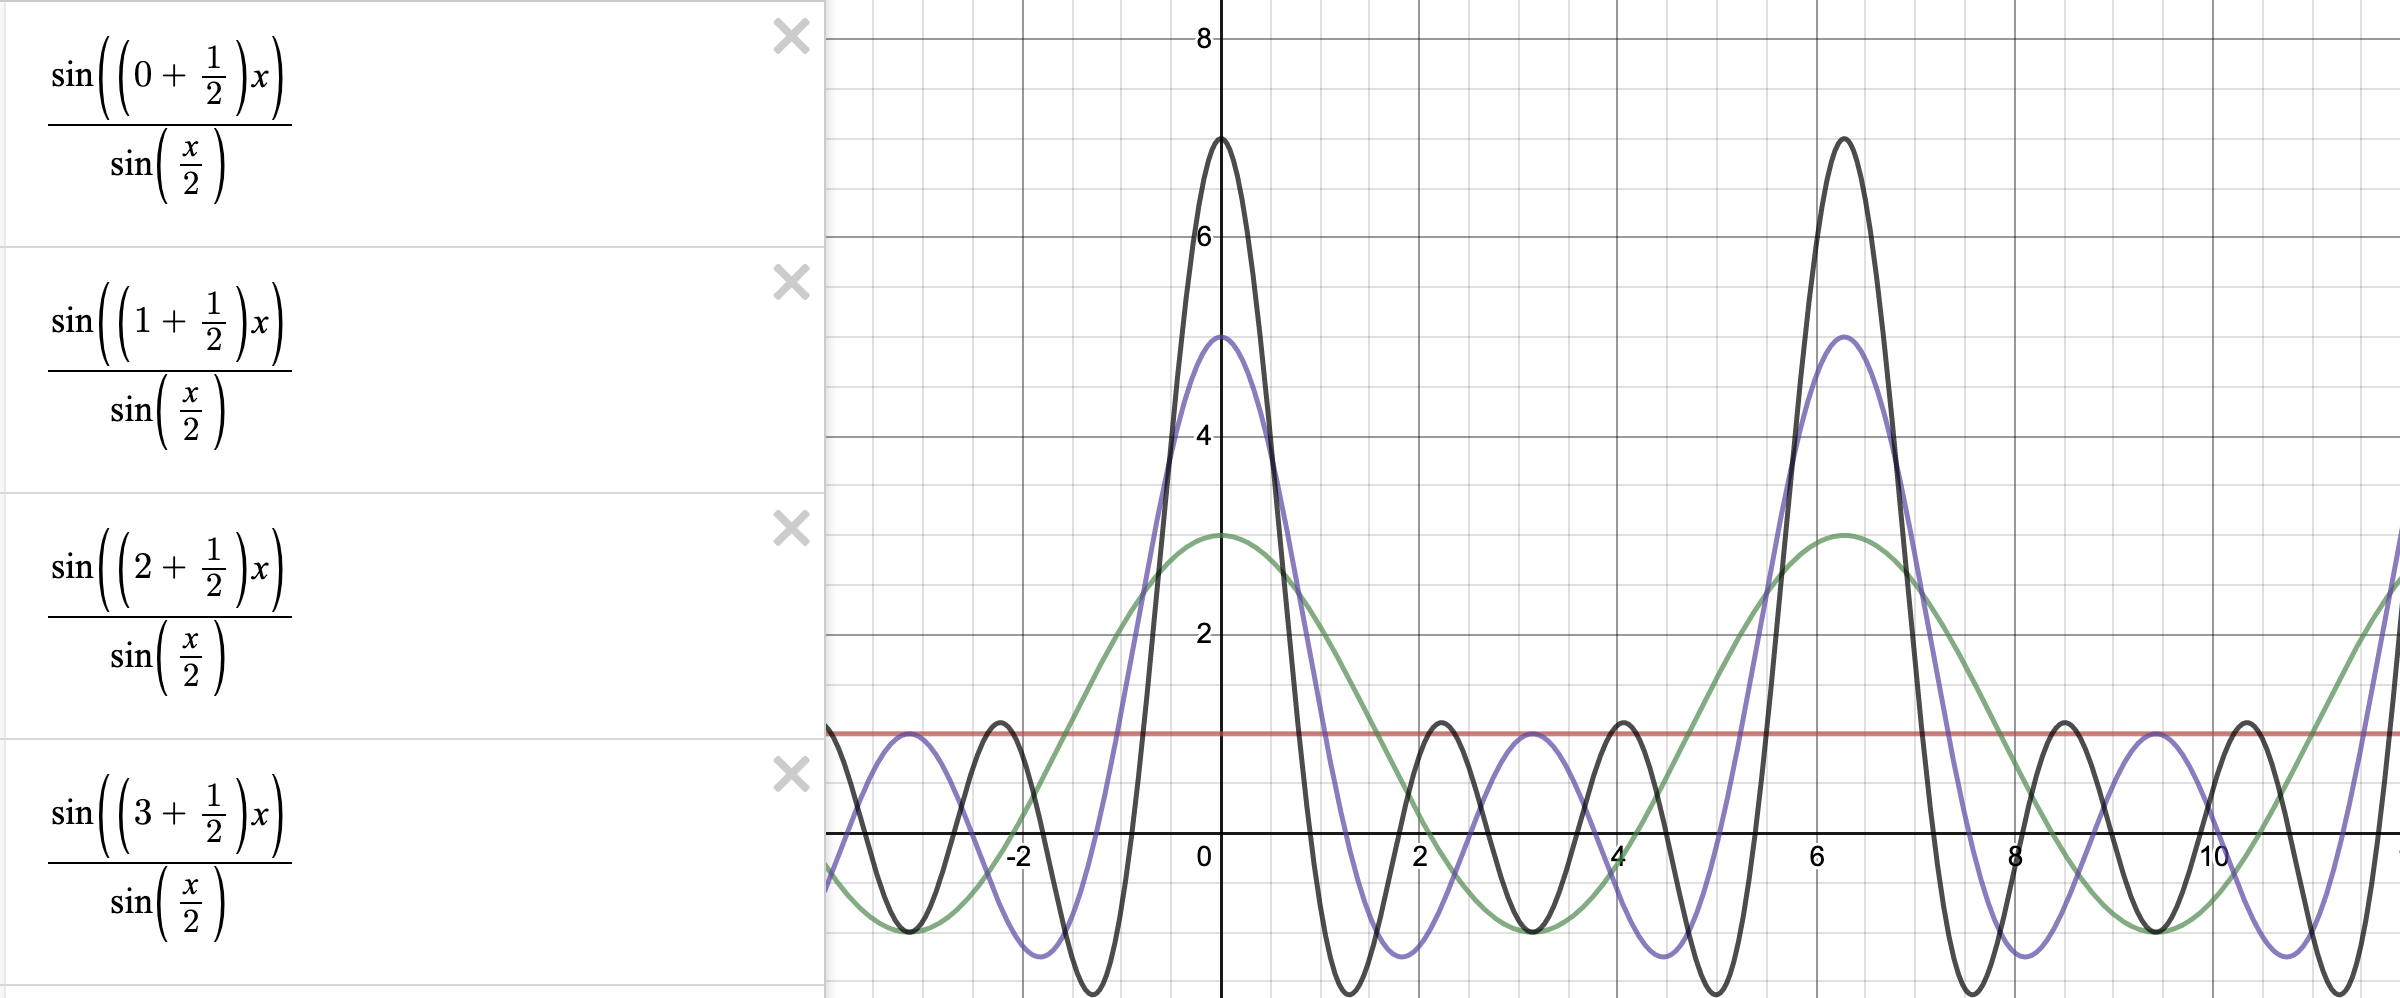
\includegraphics[scale=0.35]{dn.png}
\end{center}

Note that $$\frac{1}{2\pi} \int_{-\pi}^\pi D_N(x)dx = \frac{1}{2\pi}\int_{-\pi}^\pi \sum_{n = -N}^N e^{inx}dx = 1.$$

However, $\|D_N\|_{L^1} = \Omega(\log (N)),$ so we don't have an approximate identity sequence. 
\begin{proof}
Let $M = N + \frac{1}{2}$.
\begin{align*}
\int_{2^{k2\pi/M}}^{2^{(k+1)2\pi/M}} \frac{|\sin(Mx)|}{|\sin(x/2)|}dx &\ge \int_{2^{k2\pi/M}}^{2^{(k+1)2\pi/M}} \frac{2|\sin(Mx)|}{|x|}dx \\
&\ge 2^{-k} \frac{M}{2\pi}\int_{2^{k2\pi/M}}^{2^{(k+1)2\pi/M}} |\sin(Mx)|dx \\
&= 2^{-k} \frac{1}{2\pi}\int_{2^{k2\pi}}^{2^{(k+1)2\pi}} |\sin(y)|dy\\
&= C_0 2^{-k}2^k = C_0.
\end{align*}
So $\|D_n\| = \Omega(\log N)$.
\end{proof}

\begin{thm} There exists a function $f \in C^0(\Pi^1)$ such that $S_Nf(0) \not \rightarrow f(0)$ (and $\{S_Nf(0)\}$ unbounded).
\end{thm}
\begin{proof}
Suppose for all $f \in C^0$, $\{S_Nf(0)\}$ is bounded.
$$\ell_N(g) = S_N g(0) = \frac{1}{2\pi} \int_{-\pi}^\pi g(-y)D_N(y) dy,$$
so $\ell_N \in (C_0(\T^1))^*$.  By the Uniform Boundedness Principle, $\ell_N$ is uniformly bounded: $$\|\ell_N\|_{(C^0)^*} = \frac{1}{2\pi} \|D_N\|_1 < \infty.$$
\end{proof}
\begin{thm} Let $f \in L^1(\T)$, $x_0 \in \T, a \in \C$.  If 
$$\int _\T |f(x) - a||x - x_0|^{-1} dx < \infty,$$
then $S_Nf(x_0)\rightarrow a$.
\end{thm}
\begin{proof}
Let $g(x) = f(x - x_0)$ and reduce to the case where $x_0 = 0$.  Similarly, $g(x) = f(x) - a$ reduces to the case where $a = 0$.

So $\int |f(x)||x|^{-1} < \infty$, and we want $S_Nf(0)$.

\begin{align*}
2\pi S_Nf(0) &= \int_{-\pi}^\pi \frac{f(x)}{\sin(x/2)} \sin((N+1/2)x)dx ].\\
\end{align*}
So we have 
\begin{align*}
I &= \int_{-\pi}^\pi g(x)e^{iNx}dx \rightarrow 0,
\end{align*}
by the Riemann-Lebesgue Lemma.
\end{proof}
\begin{corollary} If $\alpha > 0$, then $S_Nf(x) \rightarrow f(x)$ for all $x$ for all $f \in \Lambda_\alpha$.
\end{corollary}
\begin{thm} Let $\alpha \in (0 ,1)$.  There exists $C_\alpha < \infty$ so that for every $f \in \Lambda_\alpha(\T)$, and for all $N$, 
$$\left\| S_Nf - f\right \|_{C^0} \le C_\alpha N^{-\alpha} \log(N + 2)\|f\|_{\Lambda_\alpha}$$
\end{thm}
\begin{proof}
We can reduce to $S_Nf(0) - f(0)$, $f(0) = 0$.

$\|f\|_{\Lambda_\alpha}$ has norms: $$\sup_{x \ne y} \frac{|f(x) - f(y)|}{|x-y|}.$$

\begin{align*}
2\pi S_Nf(0) &=\int_{-\pi}^{\pi} f(x) \frac{\sin(Mx)}{\sin(x/2)}, M = N+1/2\\
\end{align*}

Then 
$$\left |\int_{|x| \le \delta}f(x)D_N(x)\right | \le \int_{|x| \le \delta} |x|^{\alpha}\|f\|_{\Lambda_\alpha}\frac{2}{|x|}dx = C_\alpha \|f\|_{\Lambda_\alpha}\delta^{\alpha},$$
and 
\begin{align*}
\int_{\delta}^\pi \frac{f(x)}{\sin(x/2)} e^{iMx}dx &= \int_{\delta}^\pi g(x)e^{iMx} dx\\
&= \frac{1}{2} \int_{\delta}^\pi g(x)e^{iMx} - \frac{1}{2} \int_{\delta + \pi/M}^{\pi + \pi/M} g\left (x-\frac{\pi}{M}\right )e^{iMx}dx\\
&= \frac{1}{2}\int_{\delta}^\pi [g(x) - g(x-\pi/M)]e^{iMx}dx \pm \frac{1}{2} \int_{\delta}^{\delta+\pi/N} g(x - \pi/M)e^{iMx}dx\\ &\text{               }\pm \frac{1}{2} \int_{\pi}^{\pi+\pi/M} g(x-\pi/M)e^{iMx}
\end{align*}

\end{proof}
\pagebreak
\section{September 29th, 2020}
I missed this lecture.  The notes will be updated upon reviewing the lecture notes.
\pagebreak
\section{October 1st, 2020}
\subsection{Cesaro Means and Kernels}
We are discussion functions $f : \T \rightarrow \C$.  We defined the \textbf{Cesaro Means} $\sigma_N f = (n+1)^{-1}\sum_{n =0}^N S_n f$.  We showed that $\sigma_N f = f * D_n $(we used the Normalization: $f * g(x) = \frac{1}{2\pi}\int f(x-y)g(y)dy$, so that $\hat{f*g} = \hat{f}\cdot\hat{g}$.)  

Then
$$\sigma_n f = f * K_N, \hat{K}_N(n) = \begin{cases} 1 - |n|/(N+1), |n| \le N+1 \\ 0, \text{ else}\end{cases}.$$

We also have $f*V_N$, where $V_N = K_{2N+1} - K_N$.  Note that $\|V_n\|_1 \le 3.$  Note that these form an approximate identity sequence.  This is nice because it is even stays exactly at $1$from $0$ until $N+1$ and decreases linearly to $0$.  Hence $\hat{V}_N(n) \le 1$ for all $|n| \le N+1$.  Then
$$\hat{f*V_N}(n) = \hat{f}(n), |n| \le N+1.$$

We also have \textbf{Poisson Kernels}, where $0 \le r < 1$, $$P_r(x) = \sum_{n = -\infty}^\infty r^{|n|}e^{inx}= \frac{1-r^2}{1-2r\cos(x) + r^2}.$$
The denominator is $0$ if only if $\cos(x) = 1$ and $r = 1$, but $r < 1$ and $\cos(x) \Leftrightarrow x = 0$.  One can show that this is an approximate identity family.

Note that 
$$\hat{f * P_r(n)} = \hat{f} \cdot r^{|n|} \xrightarrow{|n| \rightarrow \infty} 0.$$
This is in effect like a partial sum, but instead a weighted average.

Also note the Dirichlet problem:  Given $|z| < 1$, we would like to find $u$ such that $$\begin{cases} \Delta u = 0, |z| < 1 \\ u(e^{i\theta}) = f(\theta), |z| = 1\end{cases}$$

Let $z = re^{i\theta}$, with the natural parameterization.  
Then, 
$$u(re^{i\theta}) = \sum_{n = -\infty}^{\infty} \hat{f}(n)r^{|n|} e^{in\theta}.$$

Note that $r^{|n|}e^{in\theta} = z^n$ if $n \ge 0$ and $r^{|n|}e^{in\theta} = \overline{z}^{-n}$ if $n < 0$.
We can verify that $\Delta u = 0$ for $r < 1$.  On the boundary, we have exactly $u(e^{i\theta}) = f(\theta)$.

As a final remark, note that for $f \in L^2$, $f * K_N \rightarrow f$ in $L^2$.  But $f*K_N = \sum_{|u| < N+1}(1 - \frac{|n|}{n+1})\hat{f}(n)e^{inx}$, which is a finite linear combination of the characters.  Hence, we have a corollary:
\begin{corollary} $\text{span}\{e^{inx}: n \in \Z\}$ is dense in $L^2(\T)$.
\end{corollary}
\subsection{Proof of Kolmogorov's Theorem}
\begin{thm}[Kolmogorov] There exists $f \in L^1(\T)$ so that $(S_nf(x): N \in \N)$ diverges for almost every $x \in \T$.
\end{thm}
\begin{proof}
We show that there exists $f \in L^1$ so that $\limsup_{N \rightarrow \infty} |S_N f(x)| = \infty$ almost everywhere.  If we took $f*D_n$, we can make the convolution large at a point, but it's difficult to make the $\sup$ large over many $x$.  

We wish to find $g_j$ so that $\|g_j\|_1 = 1$ and $\sup_{N} |S_Ng_j|$ is large for many $x$.  We then form 
$$\sum_{j=1}^{\infty}2^{-j} g_j,$$
which will converge in $L^1$, but the partial sums will get large.  

\begin{lemma} For any $A < \infty$, there exists a Borel probability measure $\mu$ on $\T$ so that for almost every $x \in \T$, $\sup_{N} |S_N(\mu)(x)| \ge A$.
\end{lemma}
\begin{proof}
Note that $S_N(\mu)(x) = \sum_{|n| \le N} \hat{\mu}(n)e^{inx}$ where $\hat{\mu}(n) = \frac{1}{2\pi} \int e^{-inx}d\mu(x).$ 

Let $M < \infty$.  Take $[-\pi, \pi]$ and place $M$ almost equally space points $y_j$, so that $|y_j - \frac{2\pi j}{M}| < \frac{2\pi}{4M}$ and $\{y_j\} \cup \{1\}$ are linearly independent over $\Q$.  We choose $\mu = M^{-1}\sum_{j=1}^M \delta_{y_j}.$

Then 
\begin{align*}
2\pi S_N(\mu)(x) &= M^{-1} \sum_{j=1}^M D_N(x-y_j) \\
&= M^{-1} \sum_{j}  \frac{\sin((N+1/2)(x-y_j))}{\sin(1/2(x-y_j))}.
\end{align*}
Suppose $\{y_j: 1 \le j \le m\} \cup \{1\} \cup \{x\}$ is linearly independent over $\Q$.  For each such $x$, we claim there exists $N$ so that $|S_N(\mu)(x)| \le c_0\log (M).$

Choose $N$ such that for every $j$, the sign of the numerator is the sign of the denominator, and the magnitude of the numerator is at least $1/2$ for all $j$.  We want that $\frac{N(x-y_j)}{2\pi} - (-\frac{1}{4\pi}(x-y_j))$ is approximately some prescribed value modulo $\Z$.  Hence, we would like $\{\frac{x-y_j}{2\pi} : 1 \le j \le M\}\cup \{1\}$ to be linearly independent on $\Q$.

Then, recall \textbf{Kroneker}: if $\{t_j : 1 \le j \le M\} \cup \{1\}$ are independent over $\Q$, then for any $s_j \in \R$, $\epsilon> 0$, there exists $n \in \Z$ so that $\|nt_j - s_j\|_{\pmod{\Z}} < \epsilon$, where $\pmod{\Z}$ is distance to the nearest integer.

Then,
$$(2\pi) S_N(\mu)(x) \ge \frac{1}{2M}\sum_j \frac{1}{\frac{1}{2}|x-y_j|} \ge CM^{-1}\sum_{j=1}^M |x-y_j|^{-1} \le CM^{-1} \sum_{j=1}^{M/2}(j/M)^{-1} = \log(M).$$
\end{proof}
\begin{lemma} For every $A < \infty$, $\epsilon > 0$, there exists $K < \infty$ and $\mu$, a probability measure, then
$\sup_{N \le K} |S_N(\mu)(x)| \ge A$ for all $x \in T \setminus E$ for $|E| < \epsilon$.
\end{lemma}
\begin{lemma} For all $A< \infty$, $\epsilon > 0$, there exists $K$ and a trignometric polynomial so that $\|g\|_1 \le 1$ and $\sup_{N \le K} |S_n(g)(x)| \ge A$ for all $x \in \T\setminus E$ for $|E| < \epsilon$.
\end{lemma}
\begin{proof}
Let $\mu$ be a above, $g = \mu * V_K$.  Then $\hat{g}(n) = \hat{\mu}(n)$ for $|n| \le K$.  Hence, $S_N(g) \equiv S_N(\mu)$ whenever $N \le K$.

Then $$\|g\|_1 = \|\mu * V_K\|_1 \le \|V_K\|_1 \le 3.$$ [We replace $g$ with $g/3$ to finish the proof.]
\end{proof}

\begin{lemma} Define $\tilde S_N f(x) = \sum_{n = -\infty}^{N} \hat{f}(n) e^{inx}$.  For all $A < \infty, \epsilon > 0$, there exists $K < \infty$ so that there exists a polynomial $g$ with $\|g\| \le 1$ and $\sup_{N \le K} |\tilde{S}_N (g)(x)| \ge A$ for all $x \not \in E$, for $|E| < \epsilon$.
 \end{lemma}
 
 \begin{lemma} In Lemma $11.5$, we can achieve $\hat{g}(n) = 0$ for all $n < 0$.
 \end{lemma}
 
 Finally, we prove Kolmogorov's Theorem.  We have a family of $g_\alpha$ from Lemma $11.6$ .  Set $$F(x) = \sum_{j=1}^{\infty} 2^{-j}g_{\alpha_j}(x)e^{iT_j x}.$$
 
 We choose $\alpha_j, T_j$ recursively.  Note that $\|f\|_1 < \infty$.   Choose $T_j$ greater than the largest $n \in \N$ so that there exists $\ell < j$ with $(g_{\alpha_\ell}e^{iT_\ell x})^\wedge(n) \ne 0$.  The support of the Fourier transform of $g_{\alpha_j}e^{iT_j x}$ lies to the right of the support of the fourier transform of $\sum_{\ell < j} 2^{-\ell} g_{\alpha_\ell}e^{iT_\ell x}.$
 
 Then, we choose $\alpha_j$ so that for all $x \in E_j$ where $|E_j| < 2^{-j}$, there exists $N$ so that $$|\tilde{S}_N g_{\alpha_j}(x)| \ge 2^{2^j} + \sum_{\ell < j} 2^{-\ell} \|g_{\alpha_\ell}\|_\infty,$$
 and $\tilde{S}_N(g_{\alpha_\ell})(x) = g_{\alpha_\ell}(x)$ for $\ell < j$.
 
 Then $$\tilde{S}_N(F) = \sum_{\ell < j} 2^{-\ell}g_{\alpha_\ell}(x)e^{iT_\ell x} + \tilde{S}_N(2^{-j}g_{\alpha_j}(x)e^{iT_j x}) + \sum_{\ell > j} \tilde{S}_N(2^{-\ell}g_{\alpha_\ell} e^{iT_\ell x}(x),$$
 but the last term vanishes and the second term dominates the first.
\end{proof}
\pagebreak
\section{October 6th, 2020}
\subsection{Lucunary Series}
We define the series $\Lambda \subset \Z$ where $f(x) = \sum_{n \in \Lambda} \hat{f}(n) e^{inx}.$
Rademacher series tend to be useful when considering these types of series.

\begin{thm} ($\T = \T^1$) Let $\delta > 0$ and $\Lambda = (n_k)$ $(1+\delta)$-lacunary.  For all $p < \infty$, there exists $C = C(p, \delta) < \infty$ so that for all $a \in \ell^2$,
$$\|\sum_k a_k e^{in_k x}\|_{L^p(\T)} \le C\|a\|_{\ell^2}.$$
\end{thm}
\begin{proof}
We show
$$\int |\sum_k a_k e^{in_k x}|^p dx \le C\|a\|_{\ell^2}^l.$$

If suffices to prove this for $p = 2q$, $q \in \N$.  Then,
$$\sum_{k_1,\dots, k_q} \sum_{\ell_1, \ell_q} \prod_{j=1}^{q} a_{k_j}\prod_{m=1}^q \overline{a_{k_m}}\int_{-\pi} ^\pi e^{i(n_{k_1} + \dots -n_{\ell_q})x}dx,$$
where the integral is $0$ unless the exponent of $e$ is $0$.  

Without loss of generality, $1 + \delta$ is large relative to $q$.  Choose large $N$ and $k \equiv r \pmod N$.  Then,
$$\Lambda = \bigcup_{n=0}^{N_1} \Lambda_r.$$
It suffices to prove that $\|\sum_{k \in \Lambda_r} a_k e^{in_k x}\|_{L^{2q}} \le C\|a\|_{\ell^2}.$

We have $n_{k_1} + \dots + n_{k_q} = n_{\ell_1} + \dots + n_{\ell_q}$.  Wlog, $k_q \le k_{q-1} \le \dots \le k_1$.  Then $n_{k_1}$ is the largest, so if $\ell_1, \dots, \ell_q < k_1$, then $RHS < n_{k_1}$.
\end{proof}
\begin{thm} Let $\delta, \Lambda$ be as above.  Let $a \in \ell^2, f = \sum_k a_ke^{in_k x}.$  If $f \in L^{\infty}$, then $a \in \ell^1$.
\end{thm}

\end{document}
